% Options for packages loaded elsewhere
\PassOptionsToPackage{unicode}{hyperref}
\PassOptionsToPackage{hyphens}{url}
%
\documentclass[
]{article}
\usepackage{lmodern}
\usepackage{amssymb,amsmath}
\usepackage{ifxetex,ifluatex}
\ifnum 0\ifxetex 1\fi\ifluatex 1\fi=0 % if pdftex
  \usepackage[T1]{fontenc}
  \usepackage[utf8]{inputenc}
  \usepackage{textcomp} % provide euro and other symbols
\else % if luatex or xetex
  \usepackage{unicode-math}
  \defaultfontfeatures{Scale=MatchLowercase}
  \defaultfontfeatures[\rmfamily]{Ligatures=TeX,Scale=1}
\fi
% Use upquote if available, for straight quotes in verbatim environments
\IfFileExists{upquote.sty}{\usepackage{upquote}}{}
\IfFileExists{microtype.sty}{% use microtype if available
  \usepackage[]{microtype}
  \UseMicrotypeSet[protrusion]{basicmath} % disable protrusion for tt fonts
}{}
\makeatletter
\@ifundefined{KOMAClassName}{% if non-KOMA class
  \IfFileExists{parskip.sty}{%
    \usepackage{parskip}
  }{% else
    \setlength{\parindent}{0pt}
    \setlength{\parskip}{6pt plus 2pt minus 1pt}}
}{% if KOMA class
  \KOMAoptions{parskip=half}}
\makeatother
\usepackage{xcolor}
\IfFileExists{xurl.sty}{\usepackage{xurl}}{} % add URL line breaks if available
\IfFileExists{bookmark.sty}{\usepackage{bookmark}}{\usepackage{hyperref}}
\hypersetup{
  pdftitle={Introducción al uso del Generador Estocástico de series sintéticas},
  pdfauthor={Alessio Bocco (boccoalessio@gmail.com); Daniel Bonhaure (danielbonhaure@gmail.com); Guillermo Podestá (gpodesta@rsmas.miami.edu)},
  hidelinks,
  pdfcreator={LaTeX via pandoc}}
\urlstyle{same} % disable monospaced font for URLs
\usepackage[margin=1in]{geometry}
\usepackage{color}
\usepackage{fancyvrb}
\newcommand{\VerbBar}{|}
\newcommand{\VERB}{\Verb[commandchars=\\\{\}]}
\DefineVerbatimEnvironment{Highlighting}{Verbatim}{commandchars=\\\{\}}
% Add ',fontsize=\small' for more characters per line
\newenvironment{Shaded}{}{}
\newcommand{\AlertTok}[1]{\textcolor[rgb]{1.00,0.00,0.00}{\textbf{#1}}}
\newcommand{\AnnotationTok}[1]{\textcolor[rgb]{0.38,0.63,0.69}{\textbf{\textit{#1}}}}
\newcommand{\AttributeTok}[1]{\textcolor[rgb]{0.49,0.56,0.16}{#1}}
\newcommand{\BaseNTok}[1]{\textcolor[rgb]{0.25,0.63,0.44}{#1}}
\newcommand{\BuiltInTok}[1]{#1}
\newcommand{\CharTok}[1]{\textcolor[rgb]{0.25,0.44,0.63}{#1}}
\newcommand{\CommentTok}[1]{\textcolor[rgb]{0.38,0.63,0.69}{\textit{#1}}}
\newcommand{\CommentVarTok}[1]{\textcolor[rgb]{0.38,0.63,0.69}{\textbf{\textit{#1}}}}
\newcommand{\ConstantTok}[1]{\textcolor[rgb]{0.53,0.00,0.00}{#1}}
\newcommand{\ControlFlowTok}[1]{\textcolor[rgb]{0.00,0.44,0.13}{\textbf{#1}}}
\newcommand{\DataTypeTok}[1]{\textcolor[rgb]{0.56,0.13,0.00}{#1}}
\newcommand{\DecValTok}[1]{\textcolor[rgb]{0.25,0.63,0.44}{#1}}
\newcommand{\DocumentationTok}[1]{\textcolor[rgb]{0.73,0.13,0.13}{\textit{#1}}}
\newcommand{\ErrorTok}[1]{\textcolor[rgb]{1.00,0.00,0.00}{\textbf{#1}}}
\newcommand{\ExtensionTok}[1]{#1}
\newcommand{\FloatTok}[1]{\textcolor[rgb]{0.25,0.63,0.44}{#1}}
\newcommand{\FunctionTok}[1]{\textcolor[rgb]{0.02,0.16,0.49}{#1}}
\newcommand{\ImportTok}[1]{#1}
\newcommand{\InformationTok}[1]{\textcolor[rgb]{0.38,0.63,0.69}{\textbf{\textit{#1}}}}
\newcommand{\KeywordTok}[1]{\textcolor[rgb]{0.00,0.44,0.13}{\textbf{#1}}}
\newcommand{\NormalTok}[1]{#1}
\newcommand{\OperatorTok}[1]{\textcolor[rgb]{0.40,0.40,0.40}{#1}}
\newcommand{\OtherTok}[1]{\textcolor[rgb]{0.00,0.44,0.13}{#1}}
\newcommand{\PreprocessorTok}[1]{\textcolor[rgb]{0.74,0.48,0.00}{#1}}
\newcommand{\RegionMarkerTok}[1]{#1}
\newcommand{\SpecialCharTok}[1]{\textcolor[rgb]{0.25,0.44,0.63}{#1}}
\newcommand{\SpecialStringTok}[1]{\textcolor[rgb]{0.73,0.40,0.53}{#1}}
\newcommand{\StringTok}[1]{\textcolor[rgb]{0.25,0.44,0.63}{#1}}
\newcommand{\VariableTok}[1]{\textcolor[rgb]{0.10,0.09,0.49}{#1}}
\newcommand{\VerbatimStringTok}[1]{\textcolor[rgb]{0.25,0.44,0.63}{#1}}
\newcommand{\WarningTok}[1]{\textcolor[rgb]{0.38,0.63,0.69}{\textbf{\textit{#1}}}}
\usepackage{longtable,booktabs}
% Correct order of tables after \paragraph or \subparagraph
\usepackage{etoolbox}
\makeatletter
\patchcmd\longtable{\par}{\if@noskipsec\mbox{}\fi\par}{}{}
\makeatother
% Allow footnotes in longtable head/foot
\IfFileExists{footnotehyper.sty}{\usepackage{footnotehyper}}{\usepackage{footnote}}
\makesavenoteenv{longtable}
\usepackage{graphicx,grffile}
\makeatletter
\def\maxwidth{\ifdim\Gin@nat@width>\linewidth\linewidth\else\Gin@nat@width\fi}
\def\maxheight{\ifdim\Gin@nat@height>\textheight\textheight\else\Gin@nat@height\fi}
\makeatother
% Scale images if necessary, so that they will not overflow the page
% margins by default, and it is still possible to overwrite the defaults
% using explicit options in \includegraphics[width, height, ...]{}
\setkeys{Gin}{width=\maxwidth,height=\maxheight,keepaspectratio}
% Set default figure placement to htbp
\makeatletter
\def\fps@figure{htbp}
\makeatother
\setlength{\emergencystretch}{3em} % prevent overfull lines
\providecommand{\tightlist}{%
  \setlength{\itemsep}{0pt}\setlength{\parskip}{0pt}}
\setcounter{secnumdepth}{5}

\title{Introducción al uso del Generador Estocástico de series sintéticas}
\author{Alessio Bocco (\href{mailto:boccoalessio@gmail.com}{\nolinkurl{boccoalessio@gmail.com}}) \and Daniel Bonhaure (\href{mailto:danielbonhaure@gmail.com}{\nolinkurl{danielbonhaure@gmail.com}}) \and Guillermo Podestá (\href{mailto:gpodesta@rsmas.miami.edu}{\nolinkurl{gpodesta@rsmas.miami.edu}})}
\date{15 de December de 2020}

\begin{document}
\maketitle

{
\setcounter{tocdepth}{3}
\tableofcontents
}
\hypertarget{introducciuxf3n}{%
\section{Introducción}\label{introducciuxf3n}}

El presente documento tiene como propósito proveer ejemplos de aplicación del Generador Estocástico de datos climáticos desarrollado por el SISSA. Este software es una herramienta clave para el análisis probabilista del riesgo de sequías pero por su flexibilidad puede ser usado en una multitud de aplicaciones.

Esta guía contiene solamente ejemplos de \emph{algunas} de las posibilidades y productos derivados del generador. Es un complemento de la presentación y solo se desarrollarán y replicarán algunos de los contenidos mostrados durante la misma.

\hypertarget{instalaciuxf3n-de-paquetes-necesarios}{%
\section{Instalación de paquetes necesarios}\label{instalaciuxf3n-de-paquetes-necesarios}}

Se comprueba que estén instalados los paquetes necesarios. De no ser así,
se instalarán automáticamente.

\hypertarget{creaciuxf3n-de-directorios}{%
\section{Creación de directorios}\label{creaciuxf3n-de-directorios}}

En este paso nos aseguramos de crear los directorios que contendrán los datos
de entrada para el ajuste del modelo y los resultados.

\begin{itemize}
\tightlist
\item
  /input\_data: aquí se guardarán los datos meteorológicos y los metadatos de las estaciones
\item
  /output\_data: aquí se guardarán los resultados de la simulación
\end{itemize}

Si estos directorios no existen, se crearán.

\hypertarget{generaciuxf3n-de-series-sintuxe9ticas-para-una-sola-estaciuxf3n-meteoroluxf3gica}{%
\section{Generación de series sintéticas para una sola estación meteorológica}\label{generaciuxf3n-de-series-sintuxe9ticas-para-una-sola-estaciuxf3n-meteoroluxf3gica}}

En este ejemplo veremos como se generan series sintéticas para una sola estación meteorológica condicionada por variables trimestrales. Esta configuración permite que las series generadas copien los cambios observadas en el registro histórico.

\hypertarget{crear-archivos-de-entrada}{%
\subsection{Crear archivos de entrada}\label{crear-archivos-de-entrada}}

El primer paso consiste en generar los set de datos de entrada que se descargaron al momento de instalar el paquete del generador estocástico. Estos datos son sólo a título demostrativo, si el usuario desea correr el modelo con sus propios datos deberá cambiar los objetos que se generarán en esta sección por los suyos y colocarlos en la carpeta \texttt{input\_data}.

Los archivos necesarios son:

\begin{itemize}
\tightlist
\item
  stations.csv
\item
  climate.csv
\end{itemize}

Los datos meteorológicos se dividen en dos archivos separados: \texttt{stations.csv} y \texttt{climate.csv}. Los nombres de los mismos no deben ser necesariamente iguales a los usados aquí.

Los metadatos de las estaciones se alojan en el archivo \texttt{stations.csv}. Este archivo contiene la información de las estaciones meteorológicas que serán usadas en el ajuste del modelo. Las variables que deben ser incluidas en la tabla son:

\begin{itemize}
\tightlist
\item
  station\_id: número unívoco para cada estación meteorológica. La variable debe ser de tipo \emph{integer}
\item
  latitude: latitud en grados decimales. La variable debe ser de tipo \emph{double}
\item
  longitude: longitud en grados decimales. La variable debe ser de tipo \emph{double}
\end{itemize}

La tabla puede tener más variables pero sólo se necesitan las anteriores.

A continuación se muestran la primera fila del dataset y los tipo de datos de cada una de las variables.

\begin{Shaded}
\begin{Highlighting}[]
\CommentTok{# Vista de los metadatos de la estación}
\NormalTok{knitr}\OperatorTok{::}\KeywordTok{kable}\NormalTok{(stations[}\DecValTok{1}\NormalTok{,])}
\end{Highlighting}
\end{Shaded}

\begin{tabular}{r|r|r|l|r|r|r|l}
\hline
x & y & station\_id & nombre & lat\_dec & lon\_dec & elev & pais\_id\\
\hline
5001614 & 6256841 & 87448 & Villa Reynolds Aero & -33.7181 & -65.3737 & 486 & AR\\
\hline
\end{tabular}

El objeto \textbf{stations} debe ser convertido de \emph{tibble} a \emph{sf}. El sistema de referencia espacial debe ser planar. No es necesario un sistema de referencia espacial en particular, solamente las coordenadas deben estar expresadas en metros.

\begin{Shaded}
\begin{Highlighting}[]
\CommentTok{# Convertimos el objeto stations a sf y se convierte su proyección de WGS 1984 a}
\CommentTok{# POSGAR Argentina Faja 5.}
\NormalTok{stations }\OperatorTok\StringTok{ }
\StringTok{  }\NormalTok{sf}\OperatorTok{::}\KeywordTok{st_as_sf}\NormalTok{(}\DataTypeTok{coords =} \KeywordTok{c}\NormalTok{(}\StringTok{"lon_dec"}\NormalTok{, }\StringTok{"lat_dec"}\NormalTok{), }\DataTypeTok{crs =}  \DecValTok{4326}\NormalTok{) }\OperatorTok
\StringTok{  }\NormalTok{sf}\OperatorTok{::}\KeywordTok{st_transform}\NormalTok{(}\DataTypeTok{crs =} \DecValTok{22185}\NormalTok{)}
\end{Highlighting}
\end{Shaded}

La información climática se aloja en el archivo \texttt{climate.csv}. Este archivo contiene los datos de las estaciones meteorológicas que serán usadas en el ajuste del modelo. Las variables que deben ser incluidas en la tabla son:

\begin{itemize}
\tightlist
\item
  \texttt{date}: fecha del dato. La variable debe ser de tipo \emph{date}
\item
  \texttt{station\_id}: número unívoco para cada estación meteorológica. La variable debe ser de tipo \emph{integer}
\item
  \texttt{prcp}: datos diarios de precipitación La variable debe ser de tipo \emph{double}
\item
  \texttt{tmax}: datos diarios de temperatura máxima. La variable debe ser de tipo \emph{double}
\item
  \texttt{tmin}: datos diarios de temperatura mínima. La variable debe ser de tipo \emph{double}
\end{itemize}

A continuación se muestran las primeras cinco filas del dataset y los tipos de datos de cada una de las variables.

\begin{Shaded}
\begin{Highlighting}[]
\NormalTok{knitr}\OperatorTok{::}\KeywordTok{kable}\NormalTok{(climate[}\DecValTok{1}\OperatorTok{:}\DecValTok{10}\NormalTok{,])}
\end{Highlighting}
\end{Shaded}

\begin{tabular}{l|r|r|r|r}
\hline
date & station\_id & tmax & tmin & prcp\\
\hline
1961-01-01 & 87448 & 37.4 & 13.5 & 0.6\\
\hline
1961-01-02 & 87448 & 27.4 & 14.3 & 23.9\\
\hline
1961-01-03 & 87448 & 26.6 & 13.5 & 0.0\\
\hline
1961-01-04 & 87448 & 31.0 & 11.7 & 6.0\\
\hline
1961-01-05 & 87448 & 27.0 & 14.1 & 0.0\\
\hline
1961-01-06 & 87448 & 26.3 & 11.3 & 0.0\\
\hline
1961-01-07 & 87448 & 34.1 & 12.0 & 6.7\\
\hline
1961-01-08 & 87448 & 32.8 & 15.9 & 0.0\\
\hline
1961-01-09 & 87448 & 37.6 & 16.1 & 0.0\\
\hline
1961-01-10 & 87448 & 26.9 & 4.6 & 0.0\\
\hline
\end{tabular}

Los nombres de las variables son importantes y deben ser siempre los mismos ya que el modelo las reconocerá a partir de los mismos. Los nombres deben ser los siguientes:

\begin{itemize}
\tightlist
\item
  \texttt{date} : corresponde a la fecha del día en formato \texttt{Date}. El formato de la fecha para facilitar el reconocimiento por parte de R es ``YYYY-MM-DD'', es decir, el año expresado con cuatro dígitos y luego dos dígitos para el mes y dos para el día.
\item
  \texttt{station\_id}: Identificador unívoco de cada una de las estaciones. Debe ser un número \textbf{entero}.
\item
  \texttt{tmax}: temperatura máxima diaria expresada en °C.
\item
  \texttt{tmin}: temperatura mínima diaria expresada en °C.
\item
  \texttt{prcp}: precipitación diaria expresada en mm.
\end{itemize}

El orden de las variables no es importante pero, como se mencionó, si se deben respetar los nombres de cada una. En el caso de faltantes, no se utiliza ningún valor específico para los NAs, sólo se debe dejar ese valor vacío.
Este archivo tiene un formato largo, es decir, las estaciones se deben colocar una debajo de la otra.

A continuación veremos una visualización de las temperaturas máxima y mínima de la estación elegida para el ajuste.

\begin{center}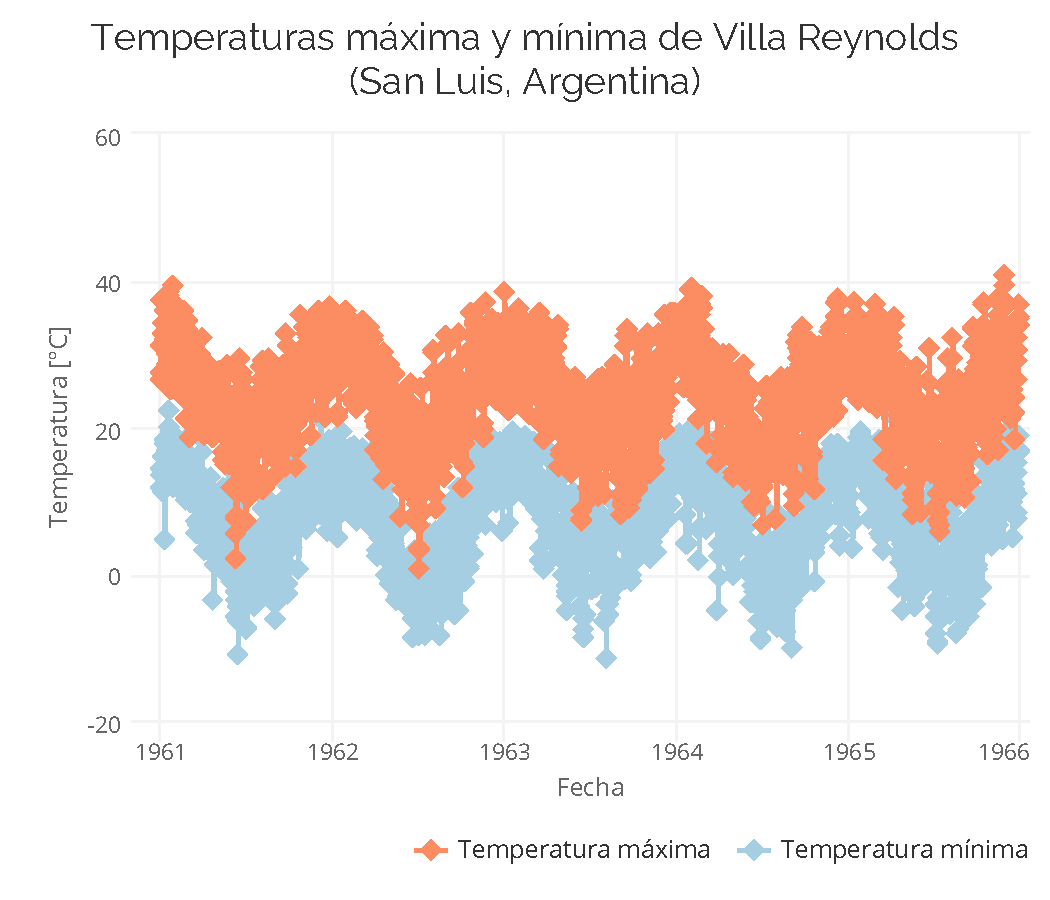
\includegraphics{Webinario_Generador_files/figure-latex/unnamed-chunk-9-1} \end{center}

Al tratarse de un modelo que ajusta condicionado por la variabilidad de baja frecuencia preexistente en los datos observados es necesario la agregación de las variables diarias en totales trimestrales de precipitación y medias trimestrales de temperaturas máxima y mínima. Esta operación puede realizarse con la función \texttt{summarise\_seasonal\_climate} incluida en el paquete.
Esta función, además de agregar los datos, permite la imputación de faltantes. Se toleran una cierta cantidad que puede ser determinada por el usuario. El método de imputación utilizado es el \texttt{imputePCA()} de la librería \texttt{missMDA} .

\begin{Shaded}
\begin{Highlighting}[]
\CommentTok{# Agregación de valores diarios }
\NormalTok{seasonal_variates <-}\StringTok{ }\NormalTok{gamwgen}\OperatorTok{::}\KeywordTok{summarise_seasonal_climate}\NormalTok{(climate, }\DataTypeTok{umbral_faltantes =} \FloatTok{0.2}\NormalTok{)}

\CommentTok{# Se muestran las primeras cinco filas}
\NormalTok{knitr}\OperatorTok{::}\KeywordTok{kable}\NormalTok{(seasonal_variates[}\DecValTok{1}\OperatorTok{:}\DecValTok{10}\NormalTok{,])}
\end{Highlighting}
\end{Shaded}

\begin{tabular}{r|r|r|r|r|r}
\hline
station\_id & year & season & seasonal\_prcp & seasonal\_tmax & seasonal\_tmin\\
\hline
87448 & 1961 & 1 & 273.7 & 30.98764 & 14.5134831\\
\hline
87448 & 1961 & 2 & 236.0 & 24.47473 & 8.4670330\\
\hline
87448 & 1961 & 3 & 11.3 & 19.04565 & 1.3456522\\
\hline
87448 & 1961 & 4 & 234.5 & 24.66235 & 7.7611765\\
\hline
87448 & 1962 & 1 & 402.4 & 29.92333 & 14.2455556\\
\hline
87448 & 1962 & 2 & 187.2 & 24.30440 & 7.9868132\\
\hline
87448 & 1962 & 3 & 50.9 & 17.21957 & -0.8978261\\
\hline
87448 & 1962 & 4 & 179.7 & 25.39560 & 7.8472527\\
\hline
87448 & 1963 & 1 & 306.8 & 29.09101 & 14.1404494\\
\hline
87448 & 1963 & 2 & 82.0 & 25.46196 & 8.5695652\\
\hline
\end{tabular}

Cabe mencionar que con esta función las valores se agregan por trimestre considerando la siguiente definición:

\begin{itemize}
\tightlist
\item
  Verano: Diciembre, Enero y Febrero
\item
  Otoño: Marzo, Abril y Mayo
\item
  Invierno: Junio, Julio y Agosto
\item
  Primavera: Septiembre, Octubre y Noviembre
\end{itemize}

Los valores también se podrían agregar siguiendo otra definición de estaciones pero en ese caso, el usuario debería hacerlo por su cuenta. Algunas funciones útiles para hacerlo son las disponibles en el paquete \texttt{lubridate} como \texttt{quarter()} que permite definir el mes de comienzo de los trimestres.
Para estas variables los nombres también son importantes por lo que deben respetarse los mostrados anteriormente.

\hypertarget{ajuste-de-los-modelos-estaduxedsticos}{%
\subsection{Ajuste de los modelos estadísticos}\label{ajuste-de-los-modelos-estaduxedsticos}}

Luego de obtener los datos observados se procede al ajuste de los modelos estadísticos: dos para temperaturas máxima y mínima y dos para precipitación. Estos modelos necesitan de datos observados diarios de variables meteorológicas. Si bien se toleran una cierta cantidad de faltantes es conveniente que las series tengan una longitud no menor a 30 años para así capturar la variabilidad climática observada.

A continuación se mostrará como ajustar los cuatro modelos estadísticos para una sola estación meteorológica condicionados por la variabilidad de baja frecuencia. La anterior es sólo uno de las configuraciones posibles y para ver más detalles de las demás posibilidades se sugiere consultar el manual completo del generador.

El ajuste del modelo local (en un punto) necesita de dos funciones: en una se define la configuración general del modelo y con la segunda se corre el modelo propiamente dicho.

Primero se crea un objeto con el control para el ajuste del simulador. Los argumentos son:

\begin{itemize}
\tightlist
\item
  \texttt{prcp\_occurrence\_threshold}: umbral de precipitación para un día lluvioso. La OMM recomienda un umbral de 0.1 mm para considerar un día como lluvioso.
\item
  \texttt{avbl\_cores}: cantidad de núcleos disponibles para la paralelización.
\item
  \texttt{planar\_crs\_in\_metric\_coords}: sistema de coordenadas planar.
\end{itemize}

\begin{Shaded}
\begin{Highlighting}[]
\NormalTok{control_fit <-gamwgen}\OperatorTok{::}\KeywordTok{local_fit_control}\NormalTok{(}
  \DataTypeTok{prcp_occurrence_threshold =} \FloatTok{0.1}\NormalTok{, }\CommentTok{# Umbral para la definición de días húmedos}
  \DataTypeTok{avbl_cores =} \DecValTok{1}\NormalTok{, }\CommentTok{# Cantidad de núcleos disponibles}
  \DataTypeTok{planar_crs_in_metric_coords =} \DecValTok{22185}\NormalTok{) }\CommentTok{# Sistema de referencia espacial (en metros)}
\end{Highlighting}
\end{Shaded}

Luego se corre el ajuste para la estación meteorológica con la función \texttt{local\_calibrate}. Los argumentos de la función son:

\begin{itemize}
\tightlist
\item
  \texttt{climate}: datos meteorológicos observados para la estación
\item
  \texttt{stations}: metadatos de las estaciones meteorológicas
\item
  \texttt{seasonal\_covariates}: datos agregados trimestrales. Si es NULL el ajuste será sin covariables y las series generadas serán estacionarias.
\item
  \texttt{control}: objeto de control
\item
  \texttt{verbose}: controla la impresión de mensajes en la consola. FALSE por defecto.
\end{itemize}

Nota: Si luego de leer este documento desean correr el generador con sus propios datos deben incluirlos en la carpeta \texttt{input\_data} y asignarle al objeto \texttt{correr.generador} el valor TRUE. Ahora esta variable es FALSE porque los resultados del ajuste ya han sido precalculados.

\begin{Shaded}
\begin{Highlighting}[]
\NormalTok{correr.generador <-}\StringTok{ }\OtherTok{FALSE}
\end{Highlighting}
\end{Shaded}

\begin{Shaded}
\begin{Highlighting}[]
\CommentTok{# Al correr la función se realiza el ajuste de los cuatro modelos para cada una de }
\CommentTok{# las estaciones. En este caso, por cuestiones de tiempo a cargar un objeto ya precalculado. }
\CommentTok{# Si el usuario desea correrlo deberá ver la nota anterior.}
\NormalTok{gamgen_fit <-}\StringTok{ }\NormalTok{gamwgen}\OperatorTok{::}\KeywordTok{local_calibrate}\NormalTok{(}\DataTypeTok{climate =}\NormalTok{ climate, }\CommentTok{# Registro histórico de variables meteorológicas}
  \DataTypeTok{stations =}\NormalTok{ stations, }\CommentTok{# Estaciones meteorológicas }
  \DataTypeTok{seasonal_covariates =} \OtherTok{NULL}\NormalTok{, }\CommentTok{# Totales trimestrales de precipitación}
  \DataTypeTok{control =}\NormalTok{ control_fit, }\CommentTok{# Objeto de control}
  \DataTypeTok{verbose =} \OtherTok{FALSE}\NormalTok{) }\CommentTok{# Impresión de mensajes en la consola.}
\end{Highlighting}
\end{Shaded}

Para esta demostración, cargamos el objeto con el ajuste del modelo ya realizado.

\begin{Shaded}
\begin{Highlighting}[]
\CommentTok{# Copiamos el archivo preajustado a nuestro directorio de trabajo}
\ControlFlowTok{if}\NormalTok{ (}\OperatorTok{!}\NormalTok{fs}\OperatorTok{::}\KeywordTok{file_exists}\NormalTok{(}\StringTok{'input_data/local/fit_local.RData'}\NormalTok{)) \{}
\NormalTok{  fs}\OperatorTok{::}\KeywordTok{file_copy}\NormalTok{(}\KeywordTok{system.file}\NormalTok{(}\StringTok{'/autorun/local'}\NormalTok{, }\StringTok{"fit_local.RData"}\NormalTok{,  }\DataTypeTok{package =} \StringTok{"gamwgen"}\NormalTok{),}
              \DataTypeTok{new_path =} \StringTok{'input_data/local/fit_local.RData'}\NormalTok{)}
\NormalTok{\}}

\CommentTok{# Cargamos el archivo recientemente creado}
\KeywordTok{load}\NormalTok{(}\StringTok{'input_data/local/fit_local.RData'}\NormalTok{)}

\CommentTok{# Clase del objeto con el ajuste del generador}
\KeywordTok{class}\NormalTok{(gamgen_fit)}
\end{Highlighting}
\end{Shaded}

\begin{verbatim}
## [1] "gamwgen"
\end{verbatim}

\begin{Shaded}
\begin{Highlighting}[]
\CommentTok{# Contenido del modelo }
\KeywordTok{names}\NormalTok{(gamgen_fit)}
\end{Highlighting}
\end{Shaded}

\begin{verbatim}
##  [1] "control"              "stations"             "climate"             
##  [4] "seasonal_covariates"  "crs_used_to_fit"      "start_climatology"   
##  [7] "fitted_models"        "models_data"          "models_residuals"    
## [10] "statistics_threshold" "exec_times"
\end{verbatim}

Dentro del objeto se guardan todo lo necesario para la simulación así como información accesoria.

\begin{itemize}
\tightlist
\item
  \texttt{control}: copia de la configuración usada para calibrar el generador
\item
  \texttt{stations}: estaciones meteorológicas utilizadas para la calibración
\item
  \texttt{climate}: datos climáticos de cada uno de las estaciones
\item
  \texttt{seasonal\_covariates}: series temporales de totales trimestrales de precipitación y medias trimestrales de temperaturas máxima y mínima.
\item
  \texttt{crs\_used\_to\_fit}: sistema de referencia espacial usado para proyectar
\item
  \texttt{start\_climatology}: climatología diaria de cada una de las variables de entrada.
\item
  \texttt{fitted\_models}: modelos ajustados, uno para cada variable: temperaturas máxima y mínima y ocurrencia y montos de precipitación.
\item
  \texttt{models\_data}: datos usados efectivamente usados para ajustar los modelos (sin NAs)
\item
  \texttt{models\_residuals}: residuos de cada uno de los modelos. Es decir, la diferencia entre el valor ajustado por el modelo (clima local) y el valor observado en el día \textbf{i}
\item
  \texttt{statistics\_threshold}: umbrales de amplitud térmica diaria por mes. Si la amplitud simulada está fuera de este rango, se repetirá la simulación para ese día a los fines de mantener la consistencia entre variables
\item
  \texttt{exec\_times}: tiempo de ejecución de cada una de las etapas del ajuste
\end{itemize}

Los umbrales de amplitudes máximos y mínimos permitidas son muy importantes para evitar que se produzcan temperaturas máximas inferiores a las mínimas. En la siguiente figura se puede ver la variabilidad mensual de cada uno de estos umbrales y el efecto del tipo de día (seco o lluvioso) sobre ellos.

\begin{center}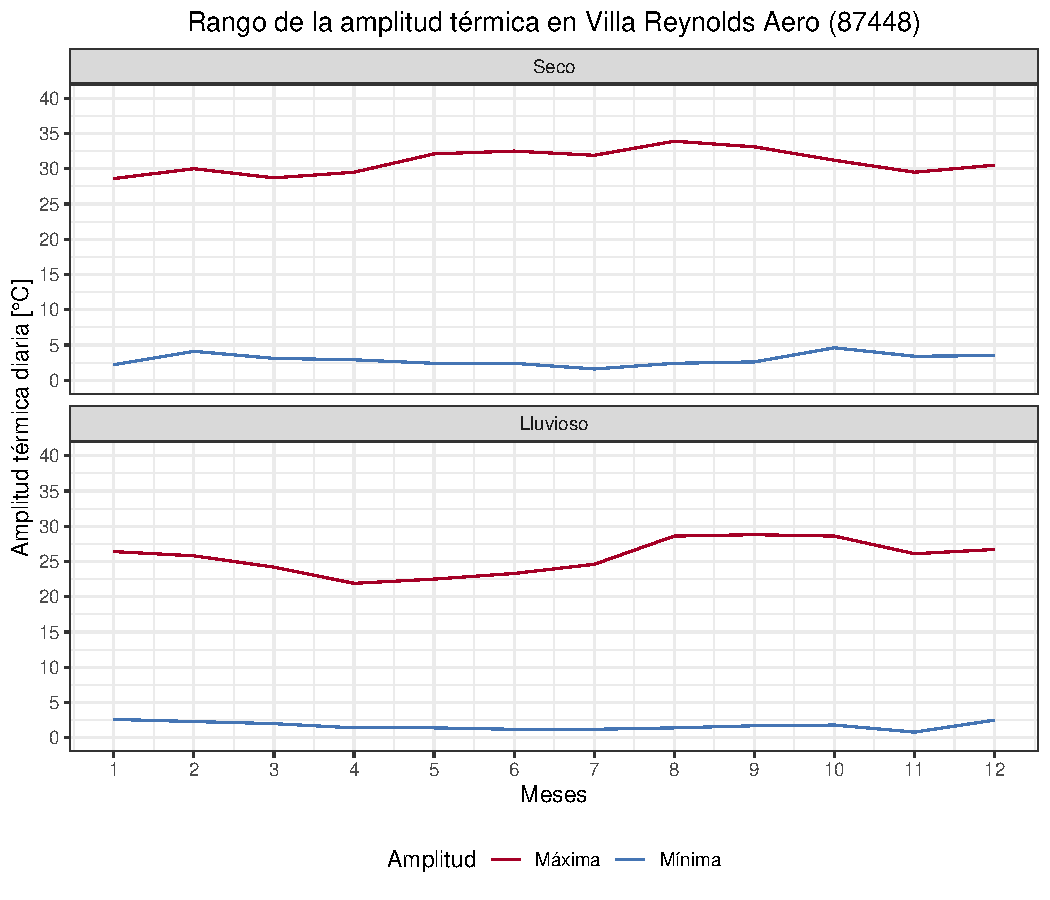
\includegraphics{Webinario_Generador_files/figure-latex/unnamed-chunk-15-1} \end{center}

Cada uno de los GAMs ajustados se almacenan en el objeto \texttt{gamgen\_fit} y pueden ser evaluados con la función \texttt{summary()}.

\begin{Shaded}
\begin{Highlighting}[]
\KeywordTok{summary}\NormalTok{(gamgen_fit}\OperatorTok{$}\NormalTok{fitted_models}\OperatorTok{$}\StringTok{`}\DataTypeTok{87448}\StringTok{`}\OperatorTok{$}\NormalTok{tmax_fit)}
\end{Highlighting}
\end{Shaded}

\begin{verbatim}
## 
## Family: gaussian 
## Link function: identity 
## 
## Formula:
## tmax ~ s(tmax_prev, tmin_prev, k = 50) + s(prcp_occ, bs = "re") + 
##     s(prcp_occ_prev, bs = "re") + s(doy, bs = "cc", k = 30) + 
##     s(SX1, SN1, k = 20) + s(SX2, SN2, k = 20) + s(SX3, SN3, k = 20) + 
##     s(SX4, SN4, k = 20)
## 
## Parametric coefficients:
##             Estimate Std. Error t value Pr(>|t|)    
## (Intercept) 25.62116    0.03189   803.4   <2e-16 ***
## ---
## Signif. codes:  0 '***' 0.001 '**' 0.01 '*' 0.05 '.' 0.1 ' ' 1
## 
## Approximate significance of smooth terms:
##                            edf Ref.df       F p-value    
## s(tmax_prev,tmin_prev) 29.9069 38.405  225.74  <2e-16 ***
## s(prcp_occ)             0.9989  1.000  930.30  <2e-16 ***
## s(prcp_occ_prev)        0.9995  1.000 2248.11  <2e-16 ***
## s(doy)                 12.6336 28.000   73.12  <2e-16 ***
## s(SX1,SN1)              3.0997  3.689   55.32  <2e-16 ***
## s(SX2,SN2)              2.0001  2.000   89.25  <2e-16 ***
## s(SX3,SN3)              4.4053  5.853   35.79  <2e-16 ***
## s(SX4,SN4)              2.0001  2.000   86.85  <2e-16 ***
## ---
## Signif. codes:  0 '***' 0.001 '**' 0.01 '*' 0.05 '.' 0.1 ' ' 1
## 
## R-sq.(adj) =  0.713   Deviance explained = 71.4%
## fREML =  58829  Scale est. = 13.964    n = 21466
\end{verbatim}

La función \texttt{summary} permite analizar los resultados del ajuste de cada uno de los modelos. Para el caso del modelo de temperatura máxima podemos ver la fórmula del GAM en la parte superior bajo el apartado \texttt{Formula} y la significancia de cada uno de los términos del modelo en la tabla inmediatamente inferior. Se puede observar que todos los términos son altamente significativos. También se incluyen como pruebas de bondad del ajuste el porcentaje de la varianza explicada por el modelo y el valor de R-ajustado.

Ahora vamos a visualizar los resultados del modelo ajustado de temperatura máxima (clima local) y la temperatura observada de la estación.

\begin{center}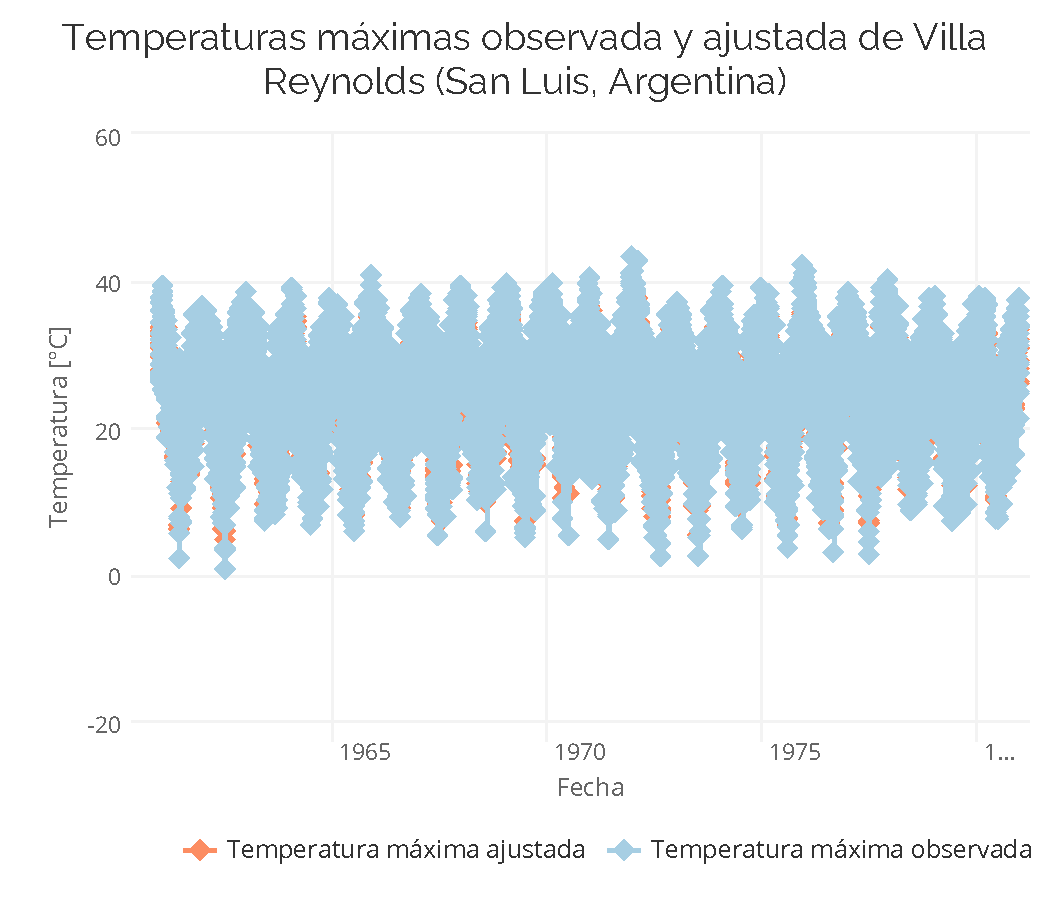
\includegraphics{Webinario_Generador_files/figure-latex/unnamed-chunk-17-1} \end{center}

Recordemos que las diferencias entre ambas curvas, los residuos del modelo, nos permitirán modelar el tiempo local que era la componente estocástica del generador.
Una vez que el los distintos modelos estadísticos de temperaturas y precipitación estén ajustados podemos proseguir a la generación de las series sintéticas.

\hypertarget{generaciuxf3n-de-series-sintuxe9ticas}{%
\section{Generación de series sintéticas}\label{generaciuxf3n-de-series-sintuxe9ticas}}

La simulación de datos también está compuesta por dos funciones. En una se especifica gran parte de la configuración de la simulación mientras que la otra realiza la simulación propiamente dicha.

Los argumentos de la función de control son:

\begin{itemize}
\tightlist
\item
  \texttt{nsim}: cantidad de simulaciones a realizar. Se debe ingresar un valor \textbf{entero} mayor o igual a 1.
\item
  \texttt{seed}: semilla. Se debe ingresar cualquier numero \textbf{entero}. No es necesario recordarlo porque se guarda junto a los resultados.
\item
  \texttt{avbl\_cores}: cantidad de núcleos disponibles para la paralelización.
\item
  \texttt{use\_spatially\_correlated\_noise}: utilizar la generación estocástica espacialmente correlacionada. Esta opción sólo es válida si en el ajuste y en la simulación se usaron más de cinco estaciones meteorológicas diferentes. Con un menor número no es posible calcular los variogramas necesarios para la generación de los campos aleatorios. Se debe introducir un \textbf{boolean} (TRUE or FALSE).
\item
  \texttt{use\_temporary\_files\_to\_save\_ram}: si se simulan muchas realizaciones o los recursos informáticos son escasos, esta opción permite guardar los resultados de cada una de las realizaciones en el disco liberando memoria RAM que quedará disponible para generar nuevas simulaciones. Al finalizar la generación todos los archivos se combinan en uno único. Se debe introducir un \textbf{boolean} (TRUE or FALSE).
\item
  \texttt{use\_temporary\_files\_to\_save\_ram}: esta opción permite eliminar los archivos temporales creados para ahorrar RAM luego de terminar la generación de todas las simulaciones. Se debe introducir un \textbf{boolean} (TRUE or FALSE).
\end{itemize}

\begin{Shaded}
\begin{Highlighting}[]
\NormalTok{control_sim <-}\StringTok{ }\NormalTok{gamwgen}\OperatorTok{::}\KeywordTok{local_simulation_control}\NormalTok{(}
  \DataTypeTok{nsim =} \DecValTok{100}\NormalTok{, }\CommentTok{# Cantidad de simulaciones a realizar}
  \DataTypeTok{seed =} \DecValTok{1234}\NormalTok{, }\CommentTok{# Semilla para que los resultados sean reproducibles}
  \DataTypeTok{avbl_cores =} \DecValTok{1}\NormalTok{, }\CommentTok{# Cantidad de núcleos disponibles a utilizar}
  \DataTypeTok{use_spatially_correlated_noise =} \OtherTok{FALSE}\NormalTok{, }\CommentTok{# Usar modelo de ruido espacialmente correlacionado}
  \DataTypeTok{use_temporary_files_to_save_ram =} \OtherTok{FALSE}\NormalTok{, }\CommentTok{# Guardar resultados intermedios para ahorrar RAM}
  \DataTypeTok{remove_temp_files_used_to_save_ram =} \OtherTok{TRUE}\NormalTok{) }\CommentTok{# Borrar los resultados intermedios creados anteriormente}
\end{Highlighting}
\end{Shaded}

Luego se procede a la simulación de datos meteorológicos. Los argumentos de la función de simulación son:

\begin{itemize}
\tightlist
\item
  \texttt{model}: objeto con el resultado de la función \texttt{local\_calibrate()}
\item
  \texttt{simulation\_locations}: objeto tipo \texttt{sf} con la ubicación de las estaciones a simular. Las estaciones usadas deben haber sido incluidas en el proceso de ajuste. No es necesario que todas estén presentes, se pueden generar series solo sobre algunas de ellas.
\item
  \texttt{start\_date}: fecha de comienzo de la generación de series sintéticas. Si no se incluyeron covariables estacionales en el ajuste, la fecha de comienzo es completamente arbitraria. Caso contrario, la fecha de comienzo no puede ser anterior al inicio de la serie de covariables, ni tampoco posterior. Se debe introducir una fecha en formato \textbf{date}
\item
  \texttt{end\_date}: fecha de fin de la generación de series sintéticas. Si no se incluyeron covariables estacionales en el ajuste, la fecha de fin es completamente arbitraria. Caso contrario, la fecha de comienzo no puede ser anterior al inicio de la serie de covariables, tampoco puede ser posterior. Se debe introducir una fecha en formato \textbf{date}
\item
  \texttt{control}: objeto de control creado con la función \texttt{control\_sim()}.
\item
  \texttt{output\_folder}: ruta al directorio donde se guardarán los resultados, tanto finales como intermedios.
\item
  \texttt{output\_filename}: nombre del archivo de salida. Para facilitar la interoperabilidad, el archivo generado es un archivo de texto en formato separado por comas (.csv)
\item
  \texttt{seasonal\_covariates}: datos agregados trimestrales. Si el ajuste se realizó con covariables, la generación también debe realizarse con ellas. Caso contrario se producirá un error. Se debe introducir un data frame con los valores agregados para las tres variables (precipitación y temperaturas máxima y mínima) pero no necesariamente deben ser los mismos a los utilizados en el ajuste. Si se desean simular tendencias de algún tipo, ya sea de un modelo de cambio climático o arbitrarias, se deben perturbar estas variables trimestrales e introducirlas aquí. Estas series si deben tener la misma longitud que el período a generar
\item
  \texttt{verbose}: controla la impresión de mensajes en la consola. FALSE por defecto.
\end{itemize}

Nota: Si luego de leer este documento desean correr el generador con sus propios datos deben incluirlos en la carpeta \texttt{input\_data} y asignarle al objeto \texttt{correr.generador} el valor TRUE. Ahora esta variable es FALSE porque los resultados del ajuste ya han sido precalculados. También debe especificarse la ruta a la carpeta \texttt{ouput\_data} para así guardar los resultados y poder correr la validación.

\begin{Shaded}
\begin{Highlighting}[]
\NormalTok{correr.generador <-}\StringTok{ }\OtherTok{FALSE}
\end{Highlighting}
\end{Shaded}

\begin{Shaded}
\begin{Highlighting}[]
\CommentTok{# Al correr la función se realiza la generación de series para cada una de las estaciones. }
\CommentTok{# En este caso, por cuestiones de tiempo, vamos a cargar un objeto con los resultados de la simulación }
\NormalTok{simulated_climate <-}\StringTok{ }\NormalTok{gamwgen}\OperatorTok{::}\KeywordTok{local_simulation}\NormalTok{(}\DataTypeTok{model =}\NormalTok{ gamgen_fit, }\CommentTok{# Objeto con los resultados del ajuste}
    \DataTypeTok{simulation_locations =}\NormalTok{ stations, }\CommentTok{# Estaciones para las cuales simular}
    \DataTypeTok{start_date =} \KeywordTok{as.Date}\NormalTok{(}\StringTok{'1961-01-01'}\NormalTok{), }\CommentTok{# Fecha de comienzo de las simulaciones}
    \DataTypeTok{end_date =} \KeywordTok{as.Date}\NormalTok{(}\StringTok{'2019-01-01'}\NormalTok{), }\CommentTok{# Fecha de fin de las simulaciones}
    \DataTypeTok{control =}\NormalTok{ control_sim, }\CommentTok{# Objeto con la configuración}
    \DataTypeTok{output_folder =} \KeywordTok{getwd}\NormalTok{(), }\CommentTok{# Directorio donde se guardarán los resultados}
    \DataTypeTok{output_filename =} \StringTok{'simulations.csv'}\NormalTok{, }\CommentTok{# Nombre del archivo de salida}
    \DataTypeTok{seasonal_covariates =}\NormalTok{ seasonal_covariates, }\CommentTok{# Covariables estacionales}
    \DataTypeTok{verbose =} \OtherTok{FALSE}\NormalTok{) }\CommentTok{# Impresión de mensajes en la consola}
\end{Highlighting}
\end{Shaded}

Esta función produce dos tipos de resultados: una lista que permanece en el ambiente de R y los datos generados que son guardados como .csv en el directorio indicado precedentemente.

\begin{Shaded}
\begin{Highlighting}[]
\CommentTok{# Copiamos el archivo preajustado a nuestro directorio de trabajo}
\ControlFlowTok{if}\NormalTok{ (}\OperatorTok{!}\NormalTok{fs}\OperatorTok{::}\KeywordTok{file_exists}\NormalTok{(}\StringTok{'output_data/local/simulated_climate_local.RData'}\NormalTok{)) \{}
\NormalTok{  fs}\OperatorTok{::}\KeywordTok{file_copy}\NormalTok{(}\KeywordTok{system.file}\NormalTok{(}\StringTok{'/autorun/local'}\NormalTok{, }\StringTok{"simulated_climate_local.RData"}\NormalTok{,  }\DataTypeTok{package =} \StringTok{"gamwgen"}\NormalTok{),}
              \DataTypeTok{new_path =} \StringTok{'output_data/local/simulated_climate_local.RData'}\NormalTok{)}
\NormalTok{\}  }
\CommentTok{# Cargamos el archivo recientemente creado}
\KeywordTok{load}\NormalTok{(}\StringTok{'output_data/local/simulated_climate_local.RData'}\NormalTok{)}

\CommentTok{# Clase del objeto con el ajuste del generador}
\KeywordTok{class}\NormalTok{(simulated_climate)}
\end{Highlighting}
\end{Shaded}

\begin{verbatim}
## [1] "list"            "gamwgen.climate"
\end{verbatim}

\begin{Shaded}
\begin{Highlighting}[]
\CommentTok{# Contenido del modelo }
\KeywordTok{names}\NormalTok{(simulated_climate)}
\end{Highlighting}
\end{Shaded}

\begin{verbatim}
## [1] "nsim"                                       
## [2] "seed"                                       
## [3] "realizations_seeds"                         
## [4] "simulation_points"                          
## [5] "output_file_with_results"                   
## [6] "output_file_fomart"                         
## [7] "rdata_file_with_fitted_stations_and_climate"
## [8] "exec_times"
\end{verbatim}

La lista contiene los siguientes objetos:

\begin{itemize}
\tightlist
\item
  \texttt{nsim}: cantidad de realizaciones.
\item
  \texttt{seed}: semilla general para toda la generación. Corresponde a la que se incluye en la función de control.
\item
  \texttt{realization\_seeds}: semillas para cada una de las realizaciones. Esto permite replicar los resultados.
\item
  \texttt{simulation\_points}: puntos donde se generaron las series sintéticas.
\item
  \texttt{output\_fil\_with\_results}: nombre del archivo con los resultados.
\item
  \texttt{output\_file\_format}: tipo de archivo de salida, en este caso .csv.
\item
  \texttt{rdata\_file\_with\_fitted\_stations\_and\_climate}: archivo \texttt{.RData} con los datos meteorológicos observados que fueron utilizados en el ajuste. También se incluyen los metadatos de cada uno de esos puntos.
\item
  \texttt{exec\_times}: tiempo de ejecución del la generación.
\end{itemize}

Ahora veremos el formato del archivo de salida que contiene las series sintéticas.

\hypertarget{resultado-de-la-generaciuxf3n}{%
\subsection{Resultado de la generación}\label{resultado-de-la-generaciuxf3n}}

\begin{Shaded}
\begin{Highlighting}[]
\CommentTok{# Se carga el set de datos simulados}
\NormalTok{simulated_climate <-}\StringTok{ }\NormalTok{readr}\OperatorTok{::}\KeywordTok{read_csv}\NormalTok{(here}\OperatorTok{::}\KeywordTok{here}\NormalTok{(}\StringTok{'output_data/local/simulated_local.csv'}\NormalTok{)) }
\end{Highlighting}
\end{Shaded}

\begin{verbatim}
## 
## -- Column specification --------------------------------------------------------
## cols(
##   realization = col_double(),
##   station_id = col_double(),
##   date = col_date(format = ""),
##   tmax = col_double(),
##   tmin = col_double(),
##   prcp = col_double()
## )
\end{verbatim}

\begin{Shaded}
\begin{Highlighting}[]
\CommentTok{# Primeras filas del objeto de salidas}
\NormalTok{knitr}\OperatorTok{::}\KeywordTok{kable}\NormalTok{(simulated_climate[}\DecValTok{1}\OperatorTok{:}\DecValTok{10}\NormalTok{,])}
\end{Highlighting}
\end{Shaded}

\begin{tabular}{r|r|l|r|r|r}
\hline
realization & station\_id & date & tmax & tmin & prcp\\
\hline
1 & 87448 & 1961-01-01 & 25.32646 & 16.46776 & 0.4817959\\
\hline
1 & 87448 & 1961-01-02 & 30.57788 & 16.09155 & 3.3716312\\
\hline
1 & 87448 & 1961-01-03 & 29.81068 & 10.72460 & 0.0000000\\
\hline
1 & 87448 & 1961-01-04 & 35.41010 & 13.63691 & 0.0000000\\
\hline
1 & 87448 & 1961-01-05 & 38.72903 & 16.95761 & 0.0000000\\
\hline
1 & 87448 & 1961-01-06 & 35.69867 & 18.40348 & 0.0000000\\
\hline
1 & 87448 & 1961-01-07 & 29.45138 & 16.21864 & 0.0000000\\
\hline
1 & 87448 & 1961-01-08 & 29.31754 & 14.14326 & 0.0000000\\
\hline
1 & 87448 & 1961-01-09 & 35.09781 & 10.85326 & 0.0000000\\
\hline
1 & 87448 & 1961-01-10 & 32.73467 & 15.62831 & 0.0000000\\
\hline
\end{tabular}

El resultado de la generación es un archivo \texttt{.csv} que contiene la siguiente información:

\begin{itemize}
\tightlist
\item
  \texttt{realization}: número de realización. Es un valor entero entre 1 y la cantidad de realizaciones definida por el usuario.
\item
  \texttt{station\_id}: número unívoco de identificación de la estación meteorológica o del punto arbitrario.
\item
  \texttt{date}: fechas de cada uno de los días de la simulación.
\item
  \texttt{tmax}: valores de temperatura máxima generada expresada en °C.
\item
  \texttt{tmin}: valores de temperatura mínima generada expresada en °C.
\item
  \texttt{prcp}: valores de precipitación diaria generada expresada en mm.
\end{itemize}

\hypertarget{diagnuxf3sticos}{%
\section{Diagnósticos}\label{diagnuxf3sticos}}

A continuación se cargan las funciones necesarias para la elaboración de los diagnósticos y se definen las variables que serán evaluadas.

\begin{Shaded}
\begin{Highlighting}[]
\CommentTok{# Funciones para realizar los diagnósticos}
\KeywordTok{source}\NormalTok{(}\StringTok{"./src/funciones_validacion.R"}\NormalTok{, }\DataTypeTok{local =}\NormalTok{ knitr}\OperatorTok{::}\KeywordTok{knit_global}\NormalTok{())}

\CommentTok{# Se definen las variables a validar}
\NormalTok{variables <-}\StringTok{ }\KeywordTok{c}\NormalTok{(}\StringTok{'tmax'}\NormalTok{, }\StringTok{'tmin'}\NormalTok{, }\StringTok{'prcp'}\NormalTok{)}

\CommentTok{# Se agrega la latitud como una variable más en el data frame con los metadatos de las estaciones}
\NormalTok{stations <-}\StringTok{ }\NormalTok{stations }\OperatorTok
\StringTok{    }\NormalTok{dplyr}\OperatorTok{::}\KeywordTok{mutate}\NormalTok{(}\DataTypeTok{lat_dec =}\NormalTok{ sf}\OperatorTok{::}\KeywordTok{st_coordinates}\NormalTok{(geometry)[,}\StringTok{'Y'}\NormalTok{])}
\CommentTok{# Estaciones usadas en el ajuste. En este ejemplo es la misma porque solo se ajustó una estación}
\NormalTok{fit_stations <-}\StringTok{ }\NormalTok{stations}
\CommentTok{# Se debe definir el umbral de lluvia}
\NormalTok{umbral.precipitacion <-}\StringTok{ }\FloatTok{0.1}
\end{Highlighting}
\end{Shaded}

El objetivo de las distintas pruebas diagnósticas es comprobar si los datos observados pueden ser considerados una realización más del generador. En otras palabras, que las series observadas no pueden distinguirse de las sintéticas. Esto no implica que tengan exactamente la misma media o desvío estándar, etc.

\begin{verbatim}
## Estacion 87448
\end{verbatim}

\begin{verbatim}
## Procesando estacion 87448
## ... variable tmax
## ... variable tmin
## ... variable prcp
## ... other plots
\end{verbatim}

\hypertarget{diagnuxf3sticos-de-precipitaciuxf3n}{%
\subsection{Diagnósticos de precipitación}\label{diagnuxf3sticos-de-precipitaciuxf3n}}

A continuación se mostrarán los distintos diagnósticos desarrollados para validar las series diarias de precipitación.

\begin{center}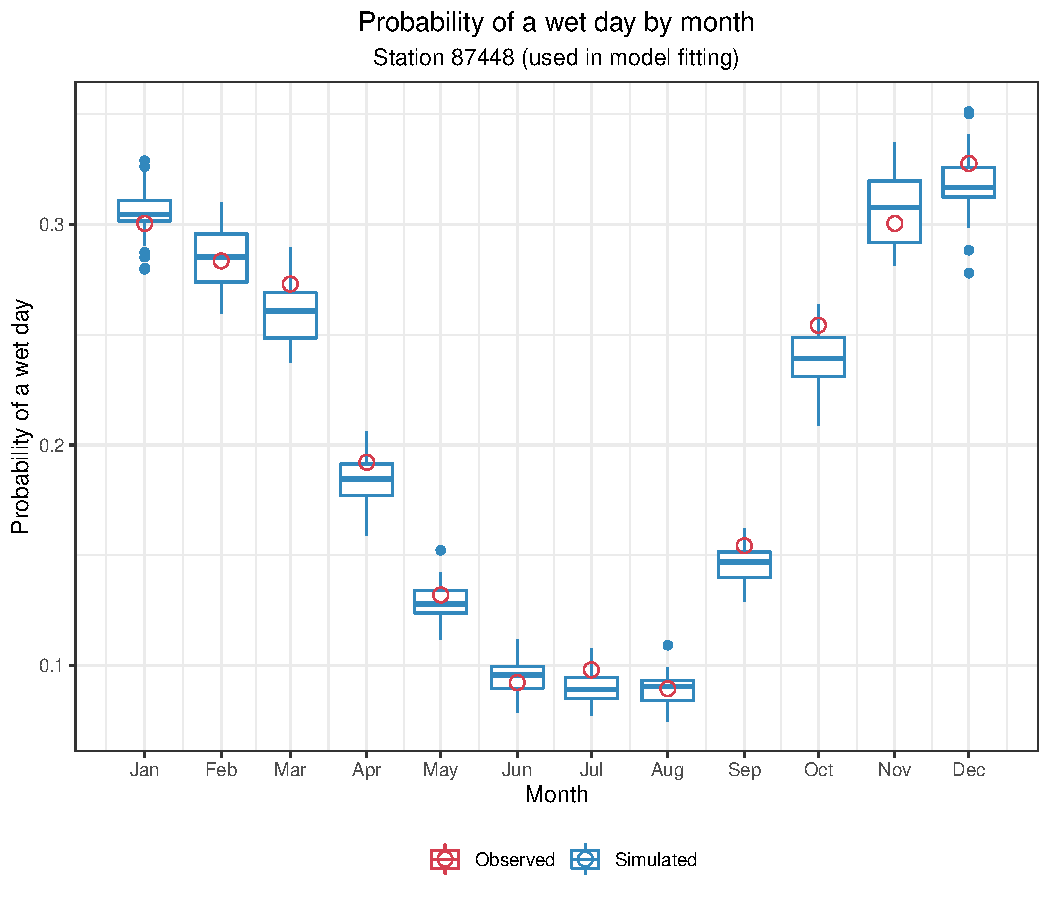
\includegraphics{Webinario_Generador_files/figure-latex/unnamed-chunk-27-1} \end{center}

Este diagrama de cajas muestra la probabilidad de ocurrencia de un día húmedo o lluvioso por mes. Las cajas corresponden a las distintas realizaciones y los puntos rojos corresponden al valor observado en la serie histórica.
Se observa un claro patrón estacional y como el generador es capaz de capturarlo. En verano, uno de cada tres días es lluvioso mientras que en invierno la probabilidad baja a menos de uno en diez.

\begin{center}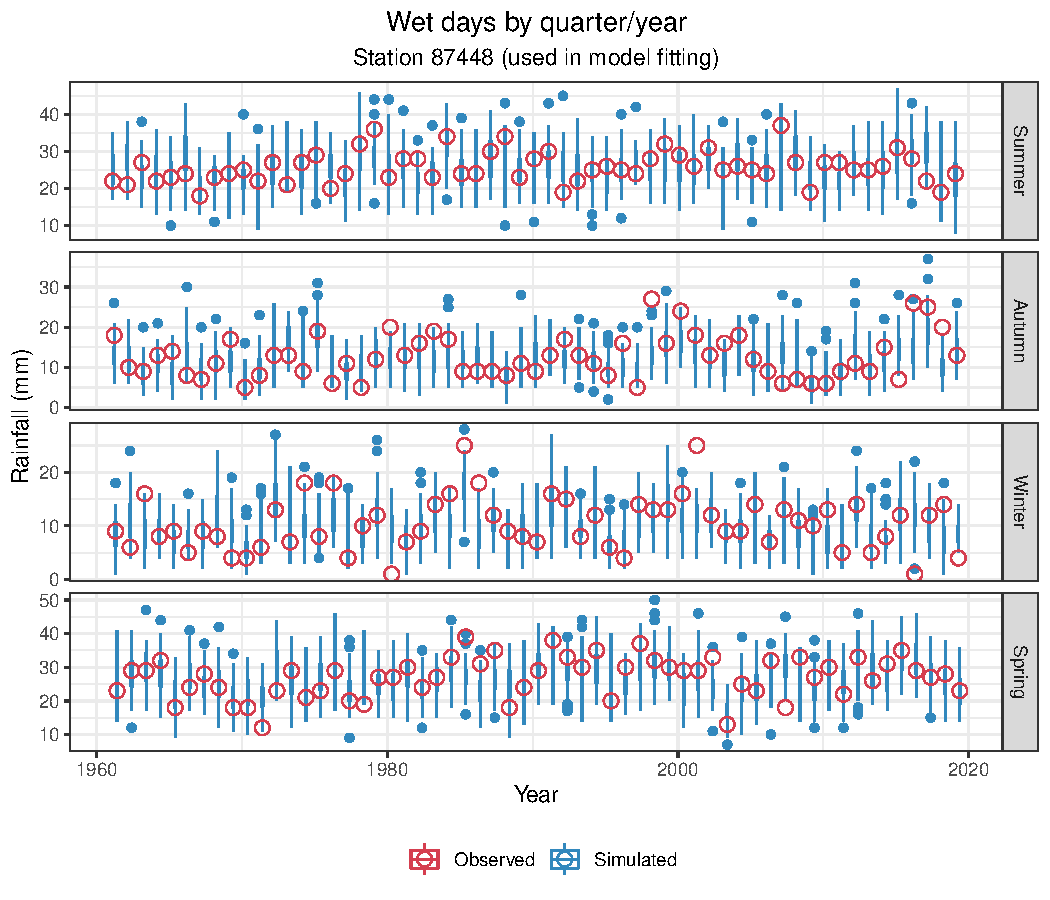
\includegraphics{Webinario_Generador_files/figure-latex/unnamed-chunk-28-1} \end{center}

Esta figura muestra la cantidad de días lluviosos por trimestre a lo largo del tiempo. Los puntos rojos corresponden a la cantidad de días lluviosos observados mientras que las cajas corresponden a las distintas realizaciones. Se observa que los puntos se encuentran dentro del rango de las distintas cajas a excepción de un trimestre excepcionalmente húmedo a principios de los 2000.

\begin{center}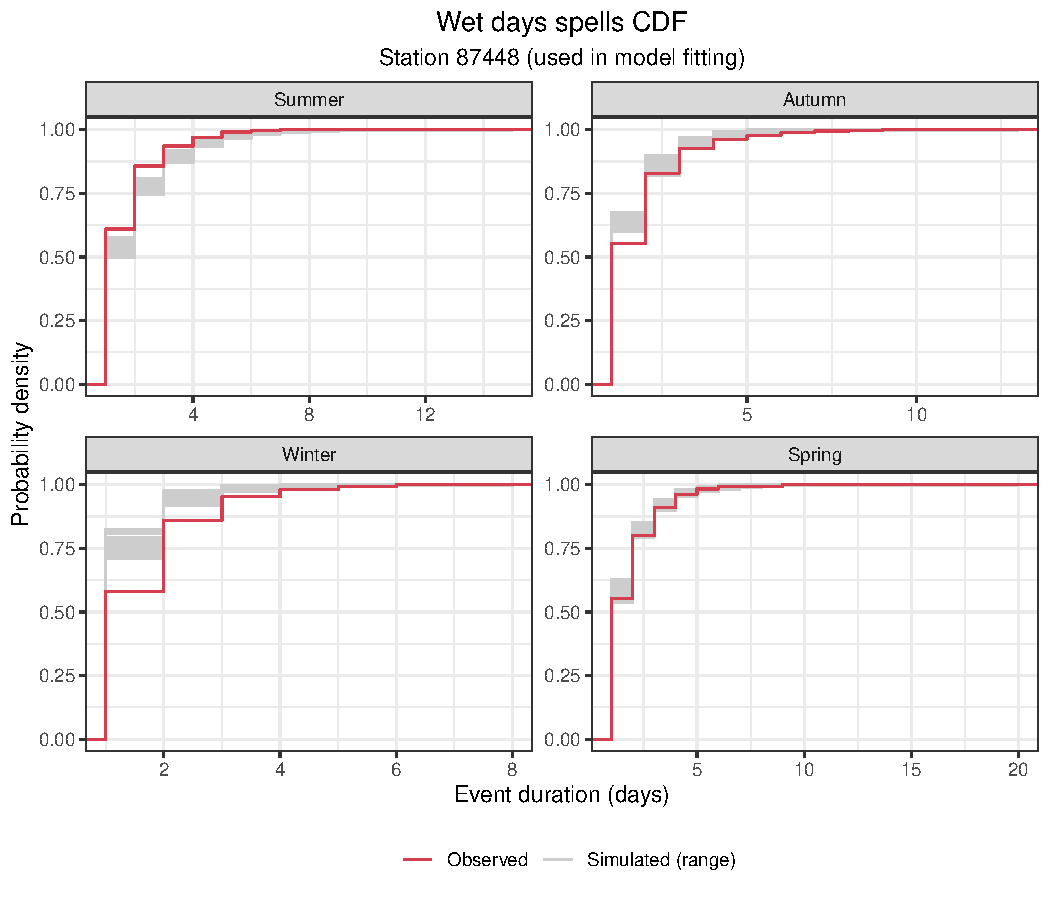
\includegraphics{Webinario_Generador_files/figure-latex/unnamed-chunk-29-1} \end{center}

Esta figura muestra la probabilidad acumulada de ocurrencia de rachas secas por trimestre. La línea roja corresponde a la probabilidad acumulada observada mientras que la envolvente gris corresponde a cada una de las realizaciones. Es un indicador muy importante para el análisis del riesgo de sequía ya que índica si la duración de los déficits hídricos es capturada o no.

\begin{center}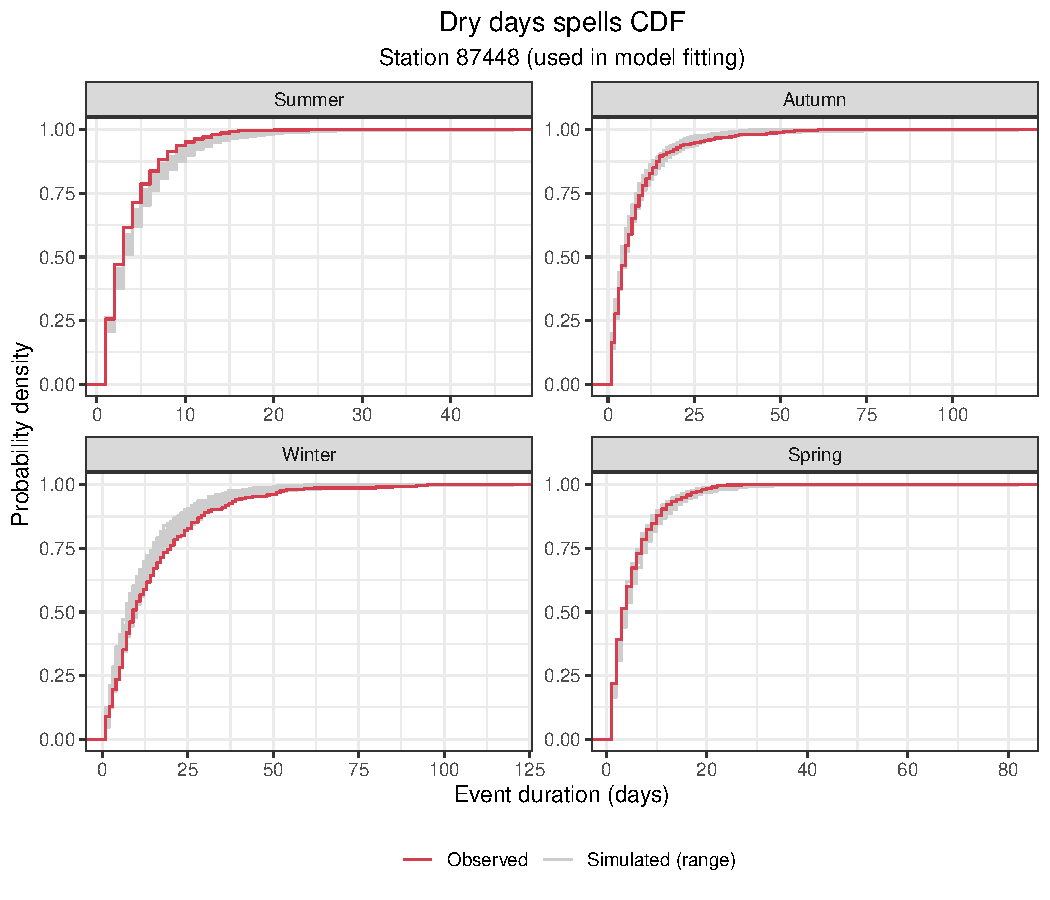
\includegraphics{Webinario_Generador_files/figure-latex/unnamed-chunk-30-1} \end{center}

Esta figura es muy similar a la anterior con la diferencia que considera las rachas secas en lugar de las secas. La línea roja corresponde a los datos observados y la envolvente gris a las distintas realizaciones. Se observa que para los cuatro trimestres la línea roja se pierde entre las realizaciones.

\begin{center}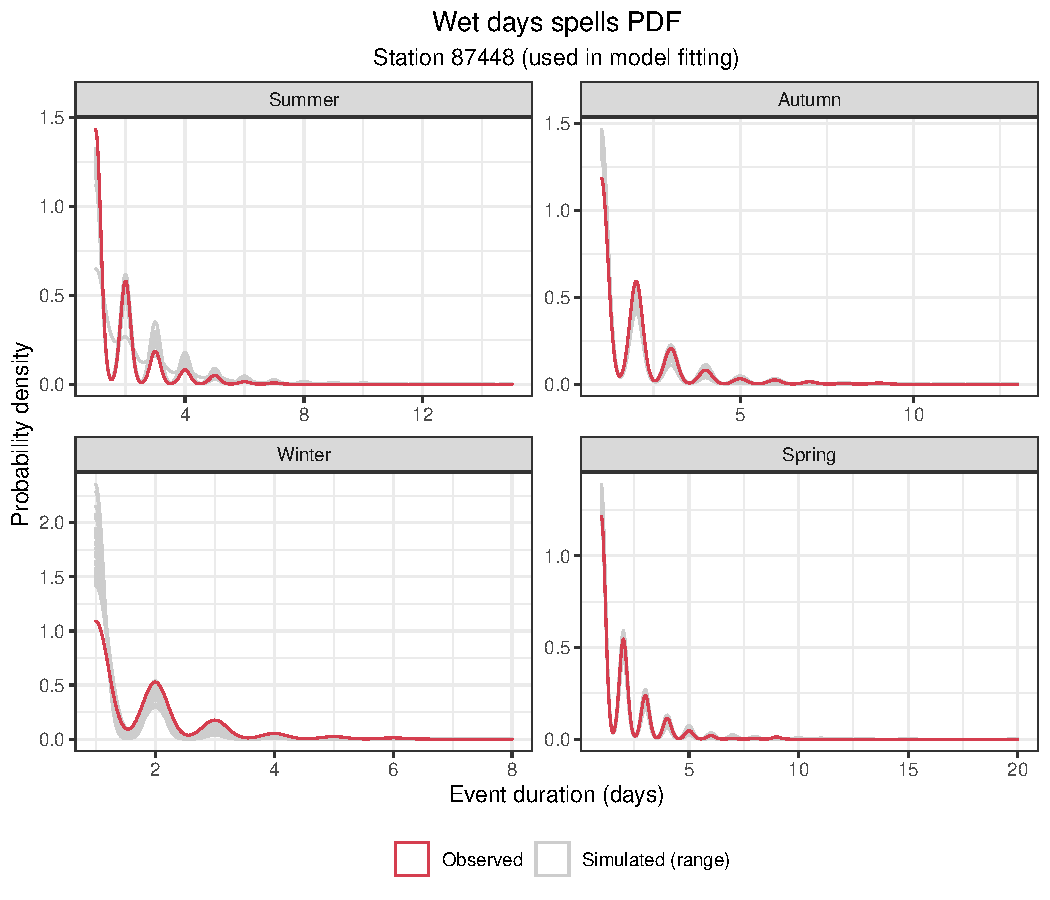
\includegraphics{Webinario_Generador_files/figure-latex/unnamed-chunk-31-1} \end{center}

Esta figura muestra la probabilidad de ocurrencia de rachas lluviosas de una determinada longitud de días por trimestre. En otras palabras, permite saber cuán frecuente es una racha lluviosa en esta estación meteorológica para cada trimestre. Las líneas rojas corresponden a la serie observada mientras que la envolvente gris a las distintas realizaciones.

\begin{center}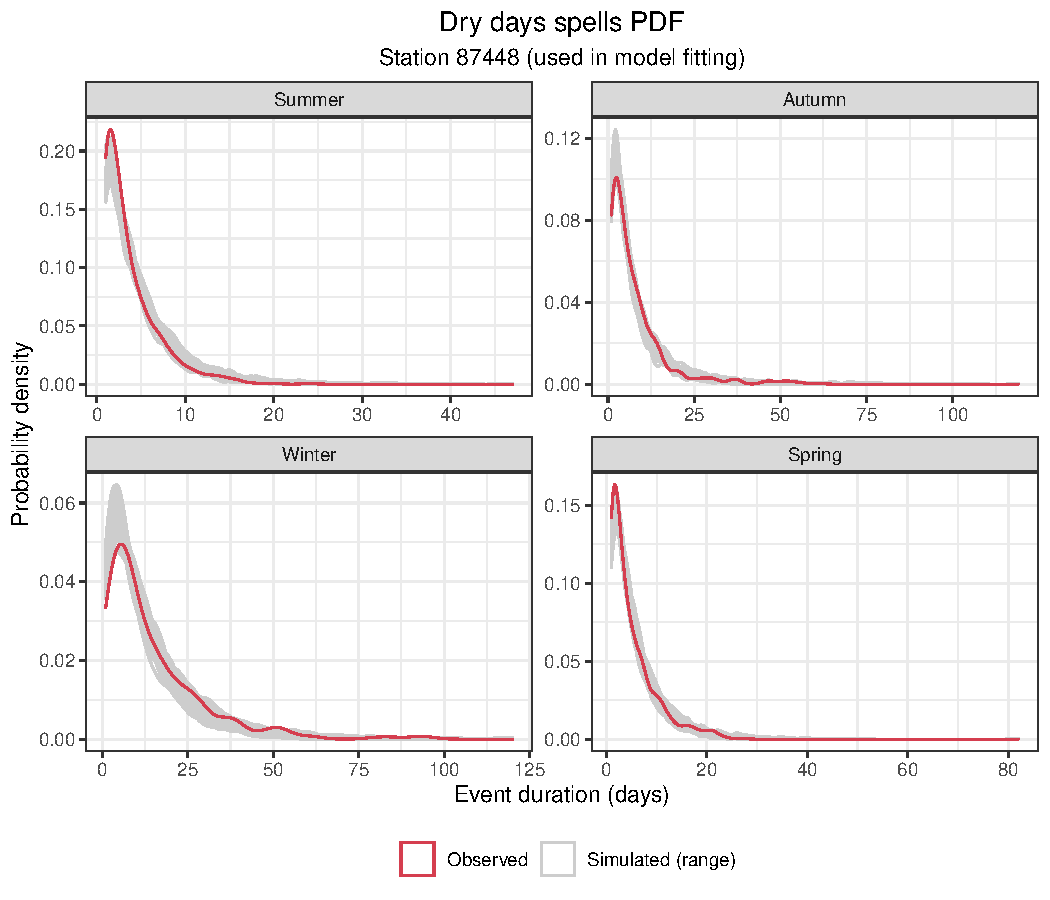
\includegraphics{Webinario_Generador_files/figure-latex/unnamed-chunk-32-1} \end{center}

Esta figura es análoga a la anterior solo que considera las rachas secas. Las líneas rojas corresponden a la serie observada y la envolvente gris a las distintas realizaciones. Se observa que las realizaciones tienen el mismo comportamiento que las series observadas y que se captura de manera correcta la variación en las rachas para los distintos trimestres. Para estudios de impacto de sequía este diagnóstico es particularmente importante ya que será uno de los determinantes principales de los déficit acumulados.

\begin{center}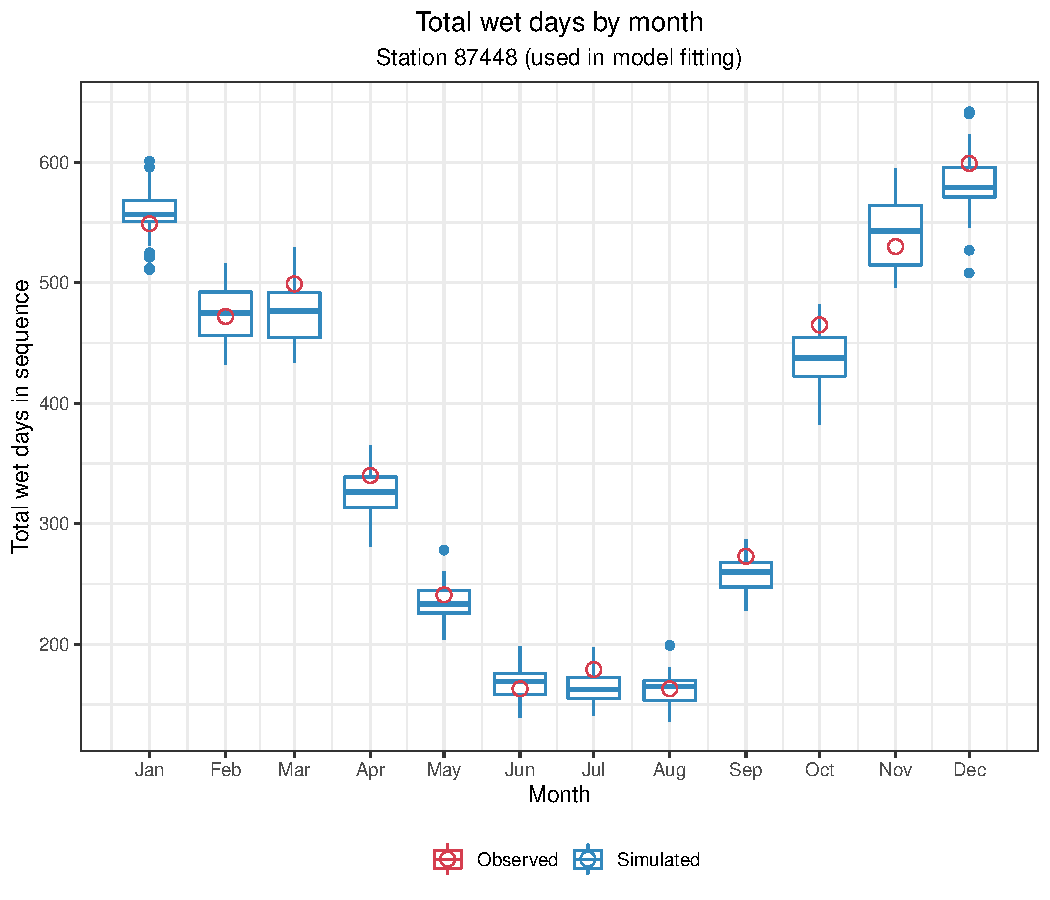
\includegraphics{Webinario_Generador_files/figure-latex/unnamed-chunk-33-1} \end{center}

Este diagrama de cajas muestra la cantidad de días lluviosos por mes y su variabilidad a lo largo del año. Las cajas corresponden a las distintas realizaciones mientras que los puntos rojos a los valores observados. La cantidad de días lluviosos por mes se acumula para todos los años del período, en este caso 57 años, es por esto que en enero los días lluviosos totalizaron aproximadamente 550. A pesar de existir una diferencia de casi 400 días entre los meses estivales e invernales, el generador es capaz de capturar están gran diferencia.

\begin{center}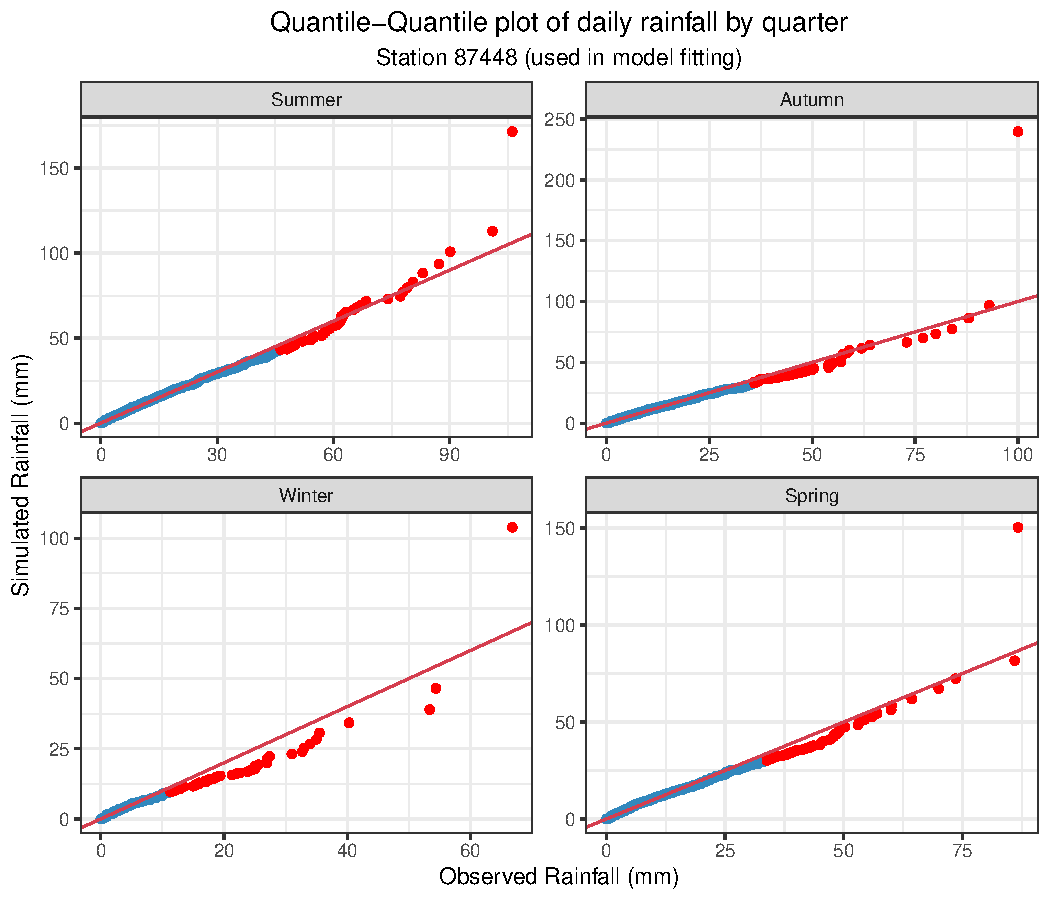
\includegraphics{Webinario_Generador_files/figure-latex/unnamed-chunk-34-1} \end{center}

Esta figura compara los cuantiles observados de precipitación diaria y los simulados por el generador por cada trimestre del año. Los puntos azules corresponden a los montos menores al percentil 99 mientras que los rojos corresponden a los montos mayores al percentil 99, es decir, a los extremos. En el eje x se ubican los cuantiles observados mientras que en el y, los simulados. El objetivo de esta prueba es que los puntos estén alineados sobre la recta 1:1 lo que indicaría que ambos cuantiles, observados y simulados, son iguales. Se observa que para casi todos los puntos, a excepción de los más extremos, la concordancia de ambas series es muy buena.

\begin{center}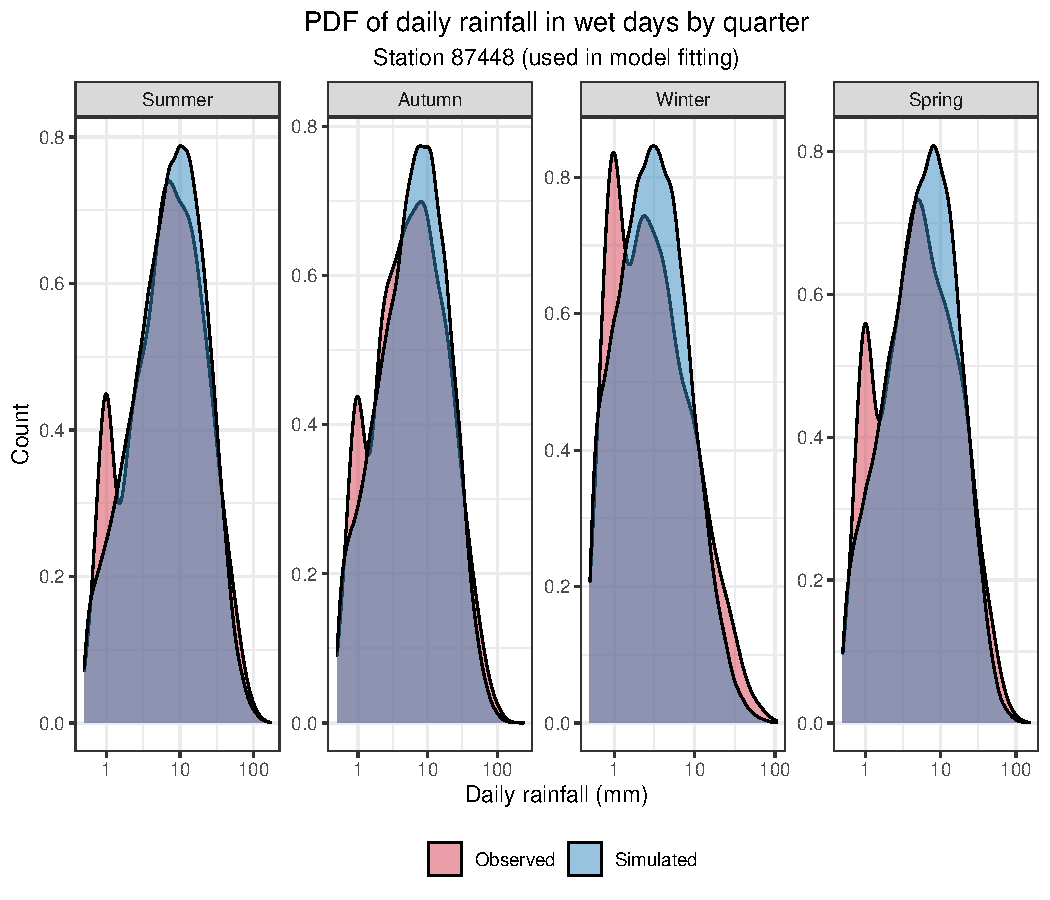
\includegraphics{Webinario_Generador_files/figure-latex/unnamed-chunk-35-1} \end{center}

Esta figura muestra la probabilidad de los montos diarios de precipitación diaria por trimestre. El área roja corresponde a los montos observados mientras que la azul, a los simulados. Cabe mencionar que la escala en el eje x es logarítmica por lo que pequeños desplazamientos sobre el eje implican grandes cambios en los montos. Se observa un buen acuerdo para las cuatro estaciones del año a excepción de los pequeños montos cercanos a un 1 mm.

\begin{center}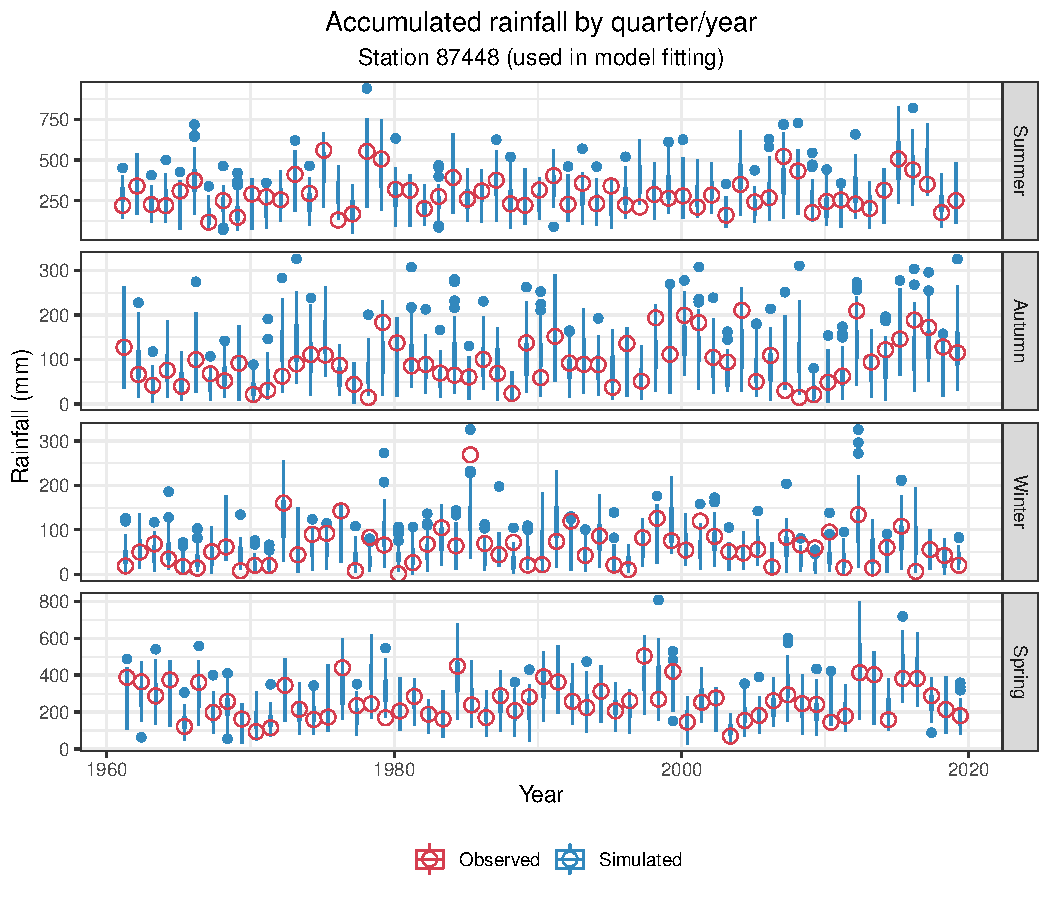
\includegraphics{Webinario_Generador_files/figure-latex/unnamed-chunk-36-1} \end{center}

Este diagnóstico compara la precipitación agregada por trimestre. Las cajas corresponden a las distintas realizaciones mientras que los puntos rojos corresponden al valor observado. Al utilizar totales trimestrales en el ajuste y la generación se producen series que copian las variaciones observadas en el registro histórico. Es decir, si el año observado tuvo precipitaciones por debajo del promedio, las distintas realizaciones tenderán a ser menores al promedio y viceversa.

\begin{center}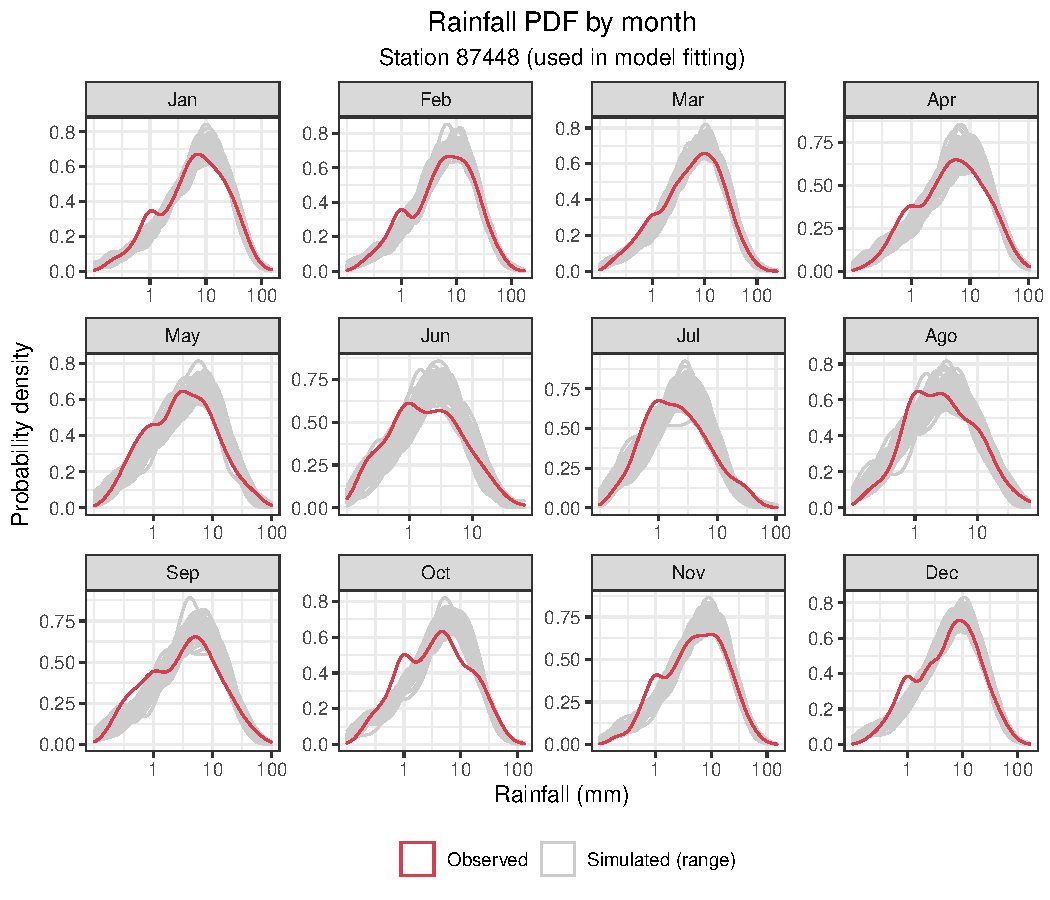
\includegraphics{Webinario_Generador_files/figure-latex/unnamed-chunk-37-1} \end{center}

Esta figura es similar a la anterior y muestra la distribución de la precipitación por mes de precipitación. La línea roja corresponde a los montos observados mientras que las grises a las distintas realizaciones. Cabe mencionar que la escala del eje x es logarítmica por lo que pequeños desplazamientos sobre el eje implican grandes cambios en los montos. Se observa un buen acuerdo para todos los meses a excepción de montos muy bajos cercanos a 1 mm.

\begin{center}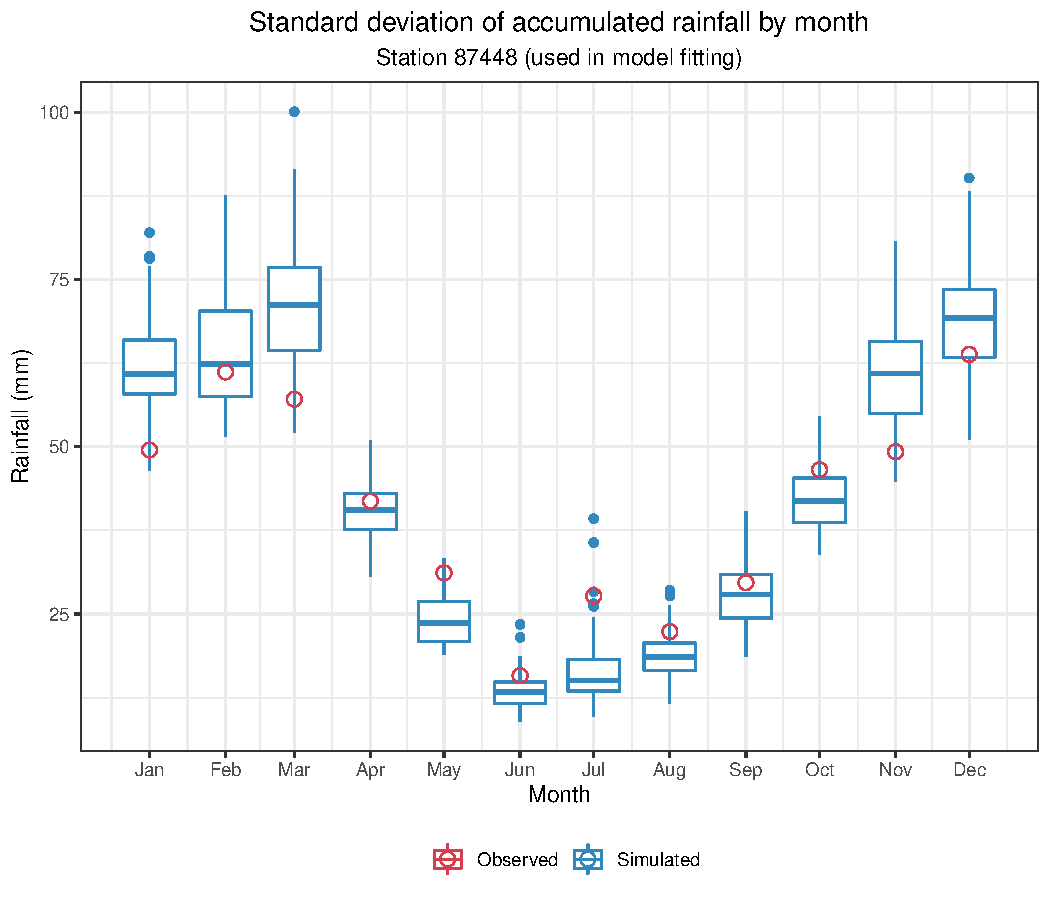
\includegraphics{Webinario_Generador_files/figure-latex/unnamed-chunk-38-1} \end{center}

Esta figura muestra la marcha mensual de los desvíos estándar de precipitación mensual. Es decir, la variabilidad de los acumulados mensuales a lo largo del año. Los puntos rojos corresponden a los valores calculados a partir de los datos observados y las cajas a las distintas realizaciones. Se observa que el generador es capaz de capturar la variabilidad intranual ya que la mediana de las cajas siguen el mismo patrón que los datos observados. Además, las cajas en los meses estivales son mas grandes lo que implica una mayor variabilidad en comparación con los meses invernales.

\begin{center}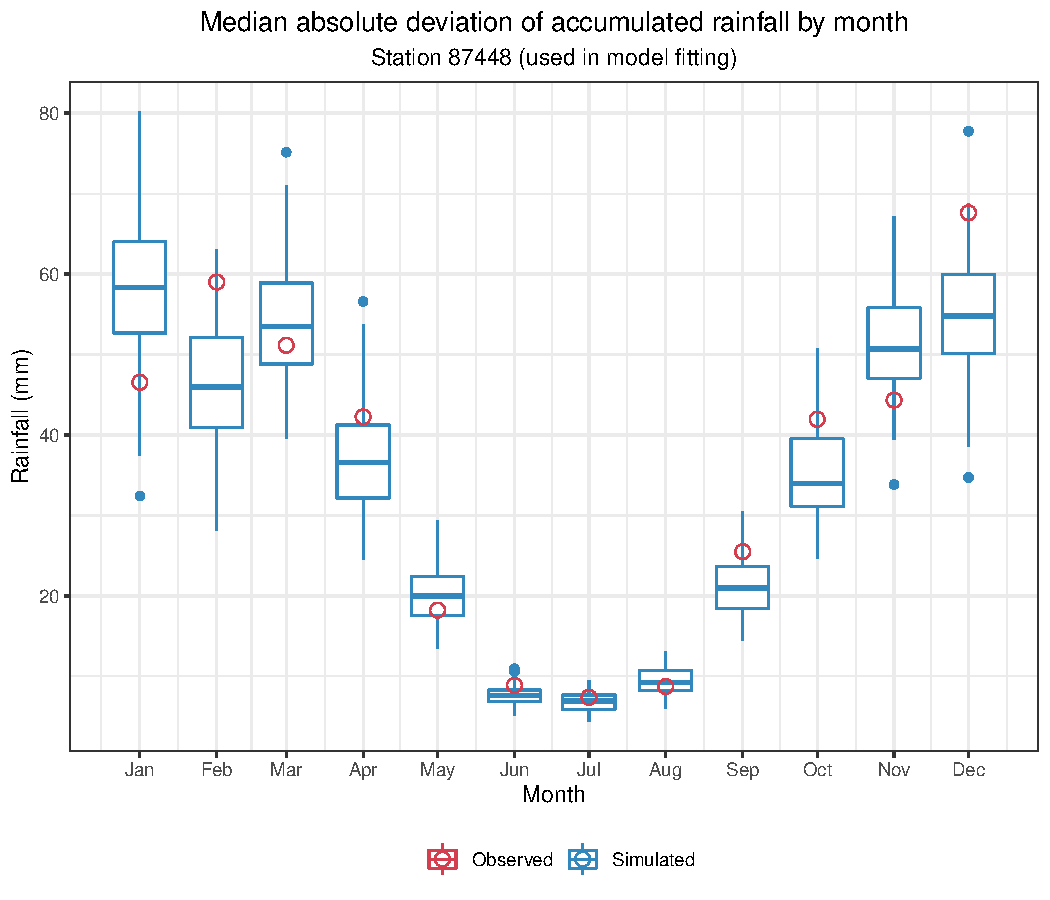
\includegraphics{Webinario_Generador_files/figure-latex/unnamed-chunk-39-1} \end{center}

Esta figura muestra otra medida de dispersión, en este caso, el desvío absoluto mediano (DMA o MAD, por sus siglas en inglés). Al igual que en el caso anterior, las cajas corresponden al MAD calculado a partir de los datos observados y las cajas a las distintas realizaciones. El buen acuerdo entre las cajas y los puntos confirma que el generador captura la variabilidad en los totales mensuales de lluvia.

\hypertarget{diagnuxf3sticos-de-temperatura-muxe1xima}{%
\subsection{Diagnósticos de temperatura máxima}\label{diagnuxf3sticos-de-temperatura-muxe1xima}}

A continuación se mostrarán los distintos diagnósticos desarrollados para validar las series diarias de temperatura máxima.

\begin{center}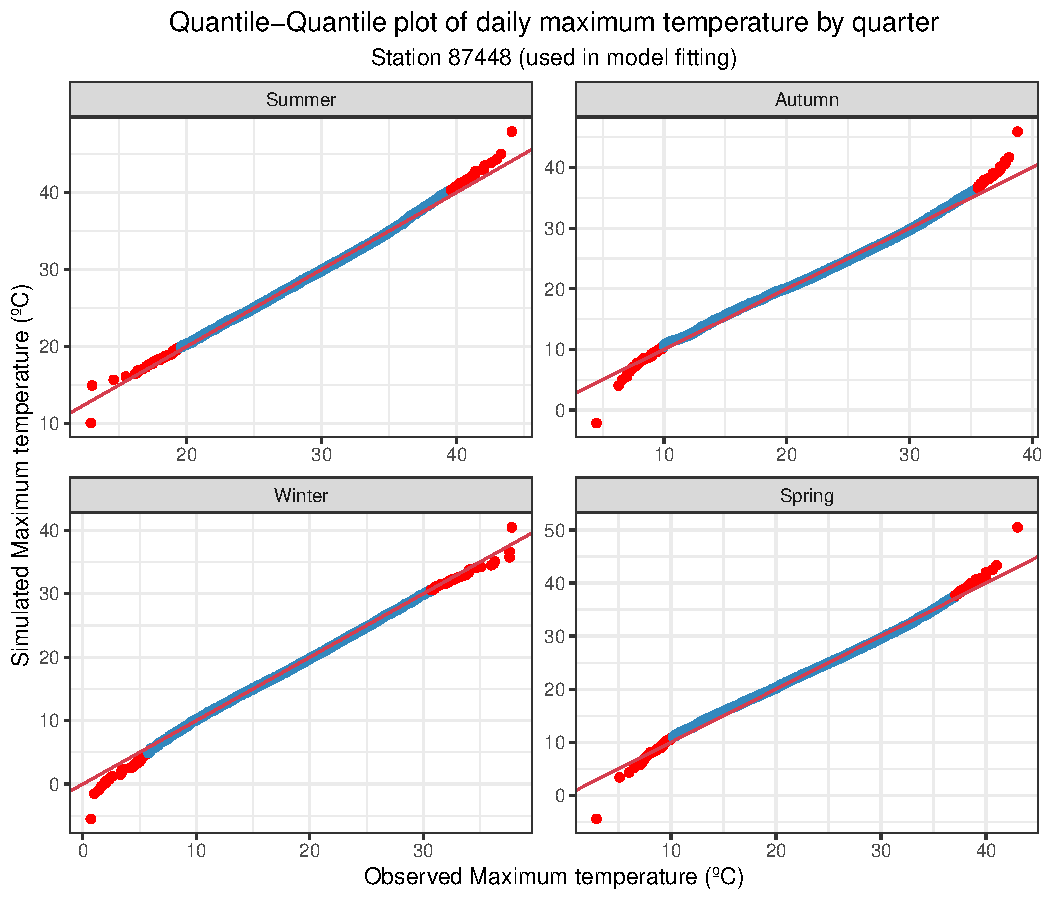
\includegraphics{Webinario_Generador_files/figure-latex/unnamed-chunk-40-1} \end{center}

En esta figura se muestra una comparación de los cuantiles observados y generados de temperatura máxima diaria por trimestre. En el eje x se encuentran los cuantiles observados mientras que en el y, los generados. Los puntos azules corresponden a los puntos cuyo valor se encuentra entre el percentil 1 y 99 y los rojos a los menores y mayores a dicho percentiles, respectivamente. El objetivo de esta prueba es verificar que todos los puntos se encuentren sobre la recta 1:1. Se observa una muy buena concordancia para los cuatros trimestres incluso en los extremos de la distribución.

\begin{center}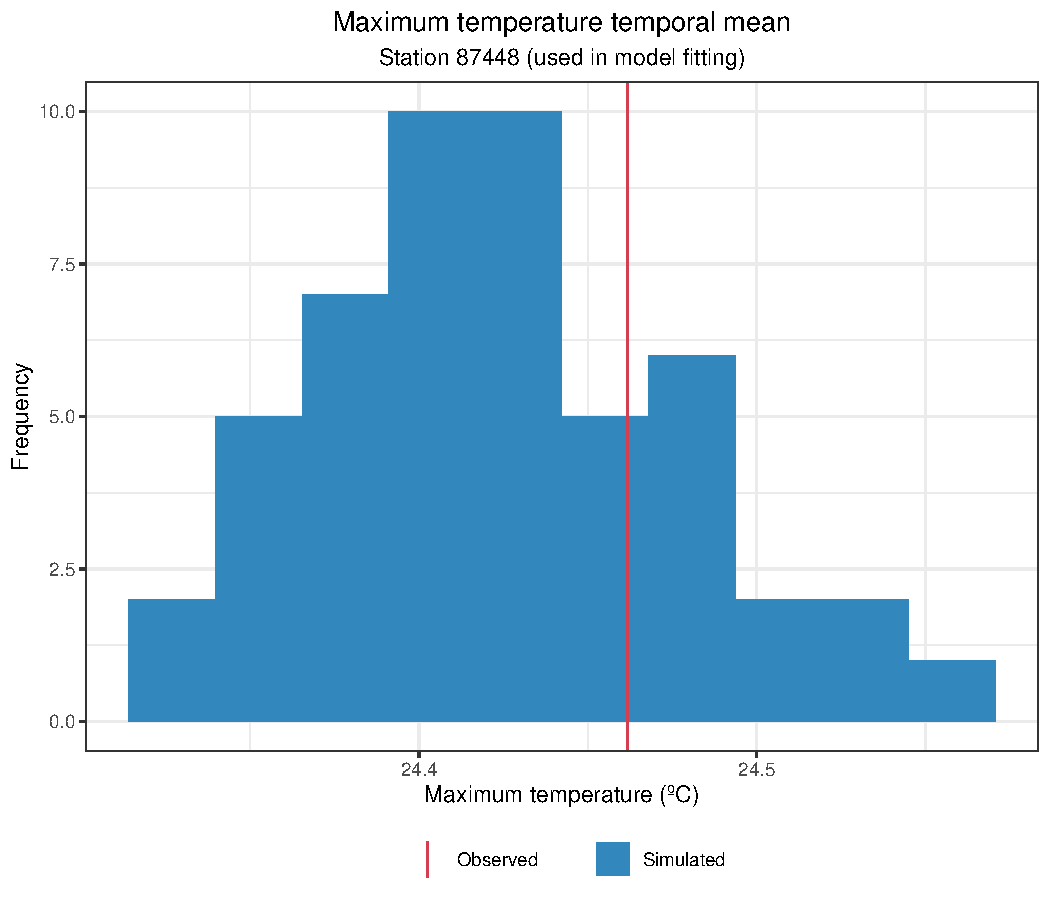
\includegraphics{Webinario_Generador_files/figure-latex/unnamed-chunk-41-1} \end{center}

Esta figura compara la temperatura máxima media de la serie observada con la de las distintas realizaciones. La línea vertical roja corresponde al valor observado mientras que las barras a las distintas realizaciones. Se observa que la medias máximas de todos las realizaciones se encuentran en un rango muy estrecho del orden de décimas de grado centígrado y que la media histórica está muy próxima a la media de las distintas realizaciones.

\begin{center}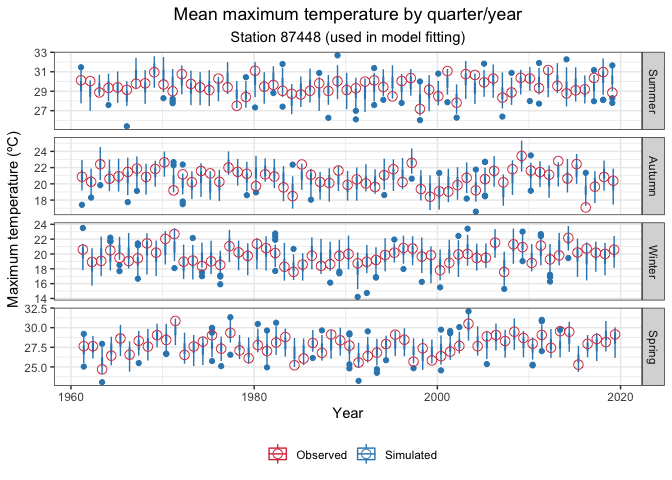
\includegraphics{Webinario_Generador_files/figure-latex/unnamed-chunk-42-1} \end{center}

Esta figura muestra la probabilidad acumulada de la temperatura máxima por trimestre del año. La línea roja corresponde a la probabilidad observada mientras que las azules, a las distintas realizaciones. Se observa que las líneas azules envuelven perfectamente a la línea roja por lo que la distribución probabilística es casi idéntica.

\begin{center}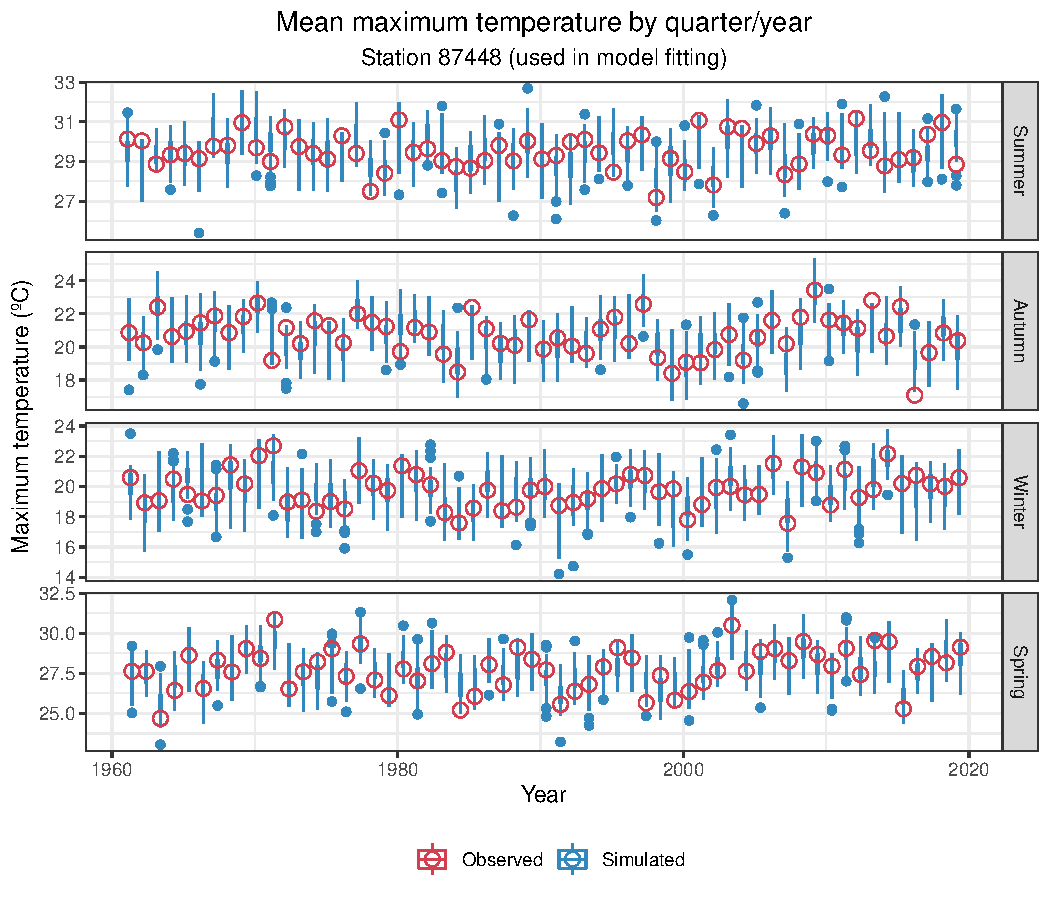
\includegraphics{Webinario_Generador_files/figure-latex/unnamed-chunk-43-1} \end{center}

Esta figura compara la variabilidad de la temperatura máxima media por trimestre a lo largo del tiempo. Los puntos rojos corresponden a las medias observadas mientras que las cajas a las distintas realizaciones. Se observa que las cajas siguen el comportamiento de los datos observados aún en años extremos.

\begin{center}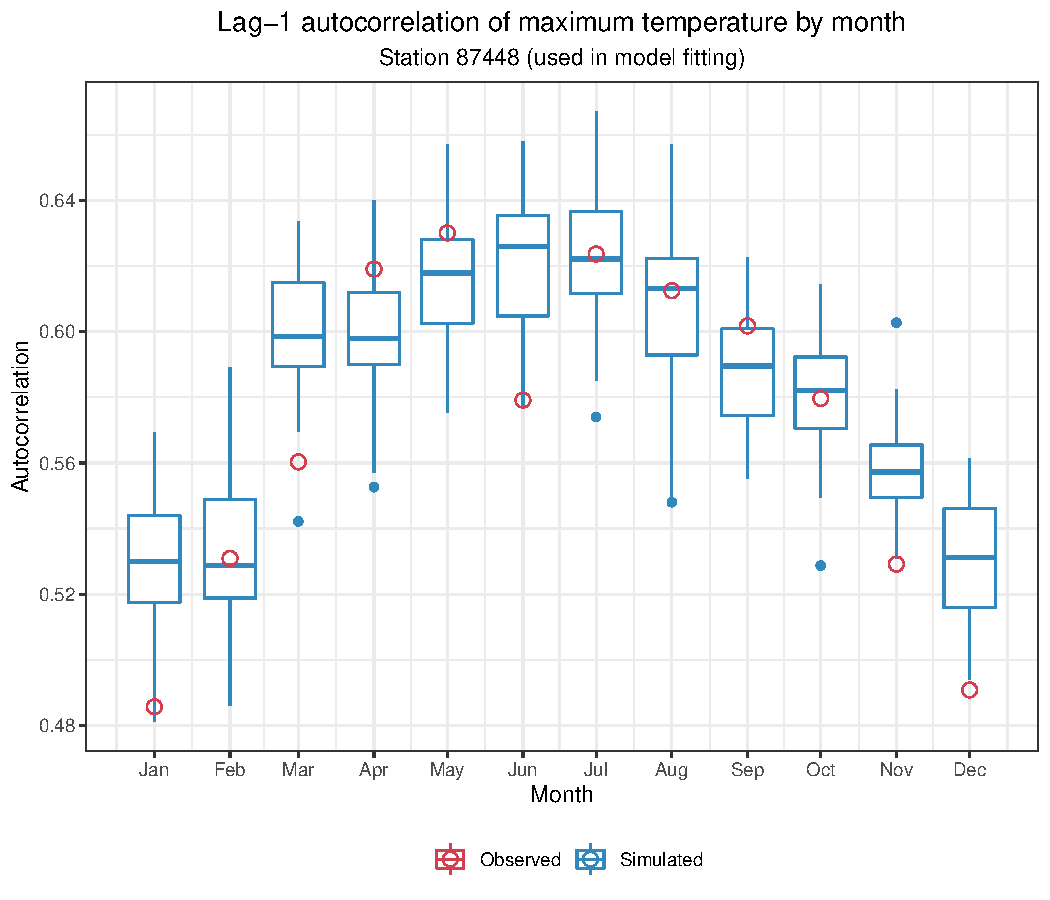
\includegraphics{Webinario_Generador_files/figure-latex/unnamed-chunk-44-1} \end{center}

Esta figura compara la autocorrelación de los valores con el lag -1 de la variable. Es decir, compara la temperatura máxima diaria del día \textbf{t} con la temperatura máxima del día \textbf{t-1}. Los puntos rojos corresponden a la autocorrelación observada mientras que las cajas a las distintas realizaciones. Se observa un patrón anual muy marcado con autocorrelaciones más altas en invierno que en verano. Este diagnóstico es muy importante para verificar si las potenciales rachas cálidas serán bien reflejadas o no ya que si un día es muy cálido, el siguiente tenderá a serlo también.

\begin{center}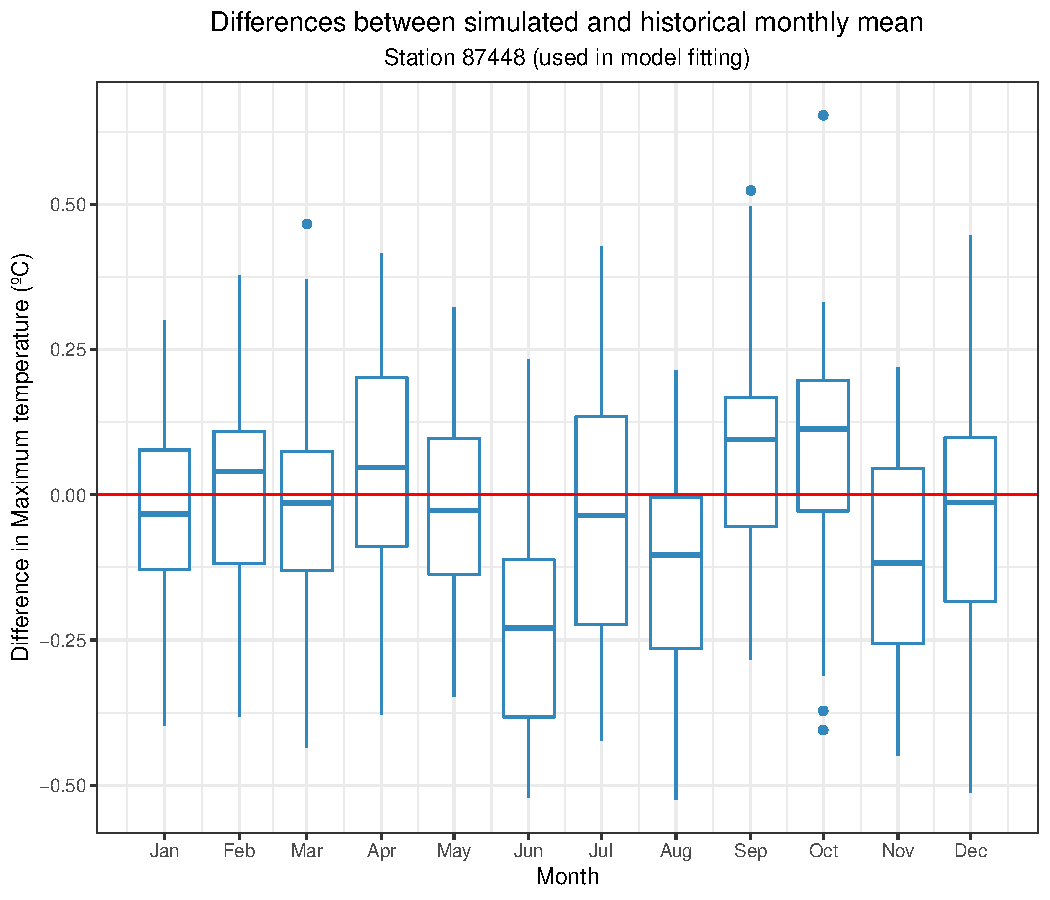
\includegraphics{Webinario_Generador_files/figure-latex/unnamed-chunk-45-1} \end{center}

Esta figura compara la media mensual calculada a partir de la series históricas con las distintas realizaciones para cada mes del año. La línea roja corresponde a una diferencia de 0 lo que quiere decir que la media observada y generada son iguales. Se observa que para casi todos los meses las cajas se encuentran sobre la línea roja a excepción de los meses de junio y agosto donde se observa un leve sesgo cálido de menos de 0.25 °C.

\begin{center}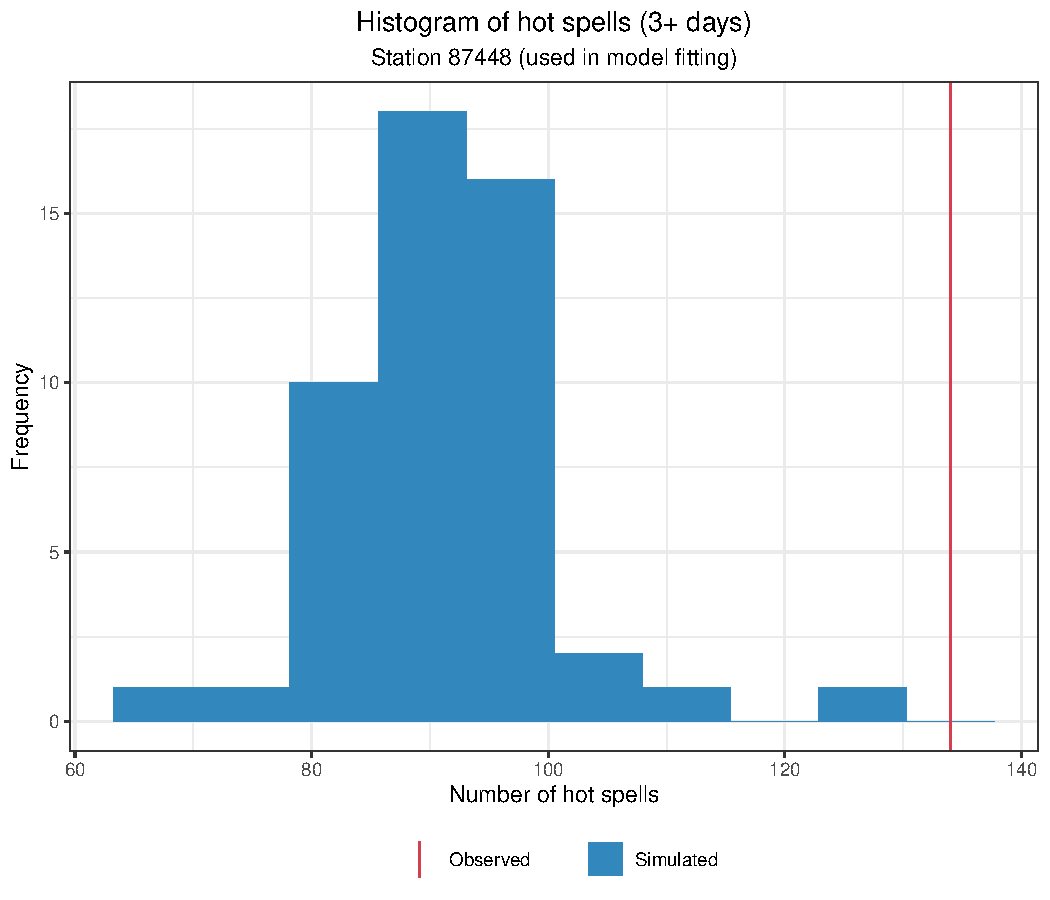
\includegraphics{Webinario_Generador_files/figure-latex/unnamed-chunk-46-1} \end{center}

Esta figura compara la distribución de la cantidad de rachas cálidas generadas con las observadas en el registro histórico. La línea roja corresponde a la cantidad de períodos cálidos totales en el registro mientras que las barras a las distintas realizaciones. Se observa que hay una subestimación en la cantidad total de rachas cálidas para esta estación.

\hypertarget{diagnuxf3sticos-de-temperatura-muxednima}{%
\subsection{Diagnósticos de temperatura mínima}\label{diagnuxf3sticos-de-temperatura-muxednima}}

A continuación se mostrarán los distintos diagnósticos desarrollados para validar las series diarias de temperatura mínima

\begin{center}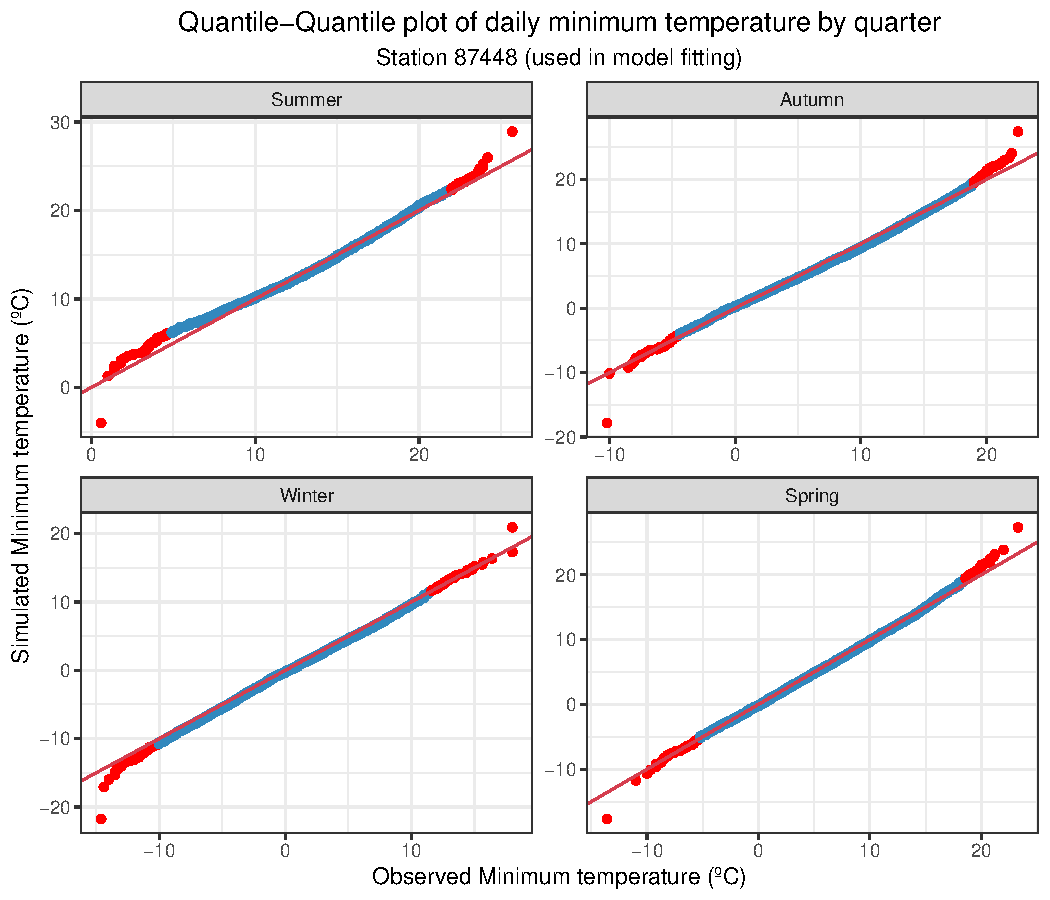
\includegraphics{Webinario_Generador_files/figure-latex/unnamed-chunk-47-1} \end{center}

En esta figura se muestra una comparación de los cuantiles observados y generados de temperatura mínima diaria por trimestre. En el eje x se encuentran los cuantiles observados mientras que en el y, los generados. Los puntos azules corresponden a los puntos cuyo valor se encuentra entre el percentil 1 y 99 y los rojos a los menores y mayores a dichos percentiles, respectivamente. El objetivo de esta prueba es verificar que todos los puntos se encuentren sobre la recta 1:1. Se observa una muy buena concordancia para los cuatro trimestres incluso en los extremos de la distribución. Solo algunos puntos son subestimados en el extremo inferior de la distribución.

\begin{center}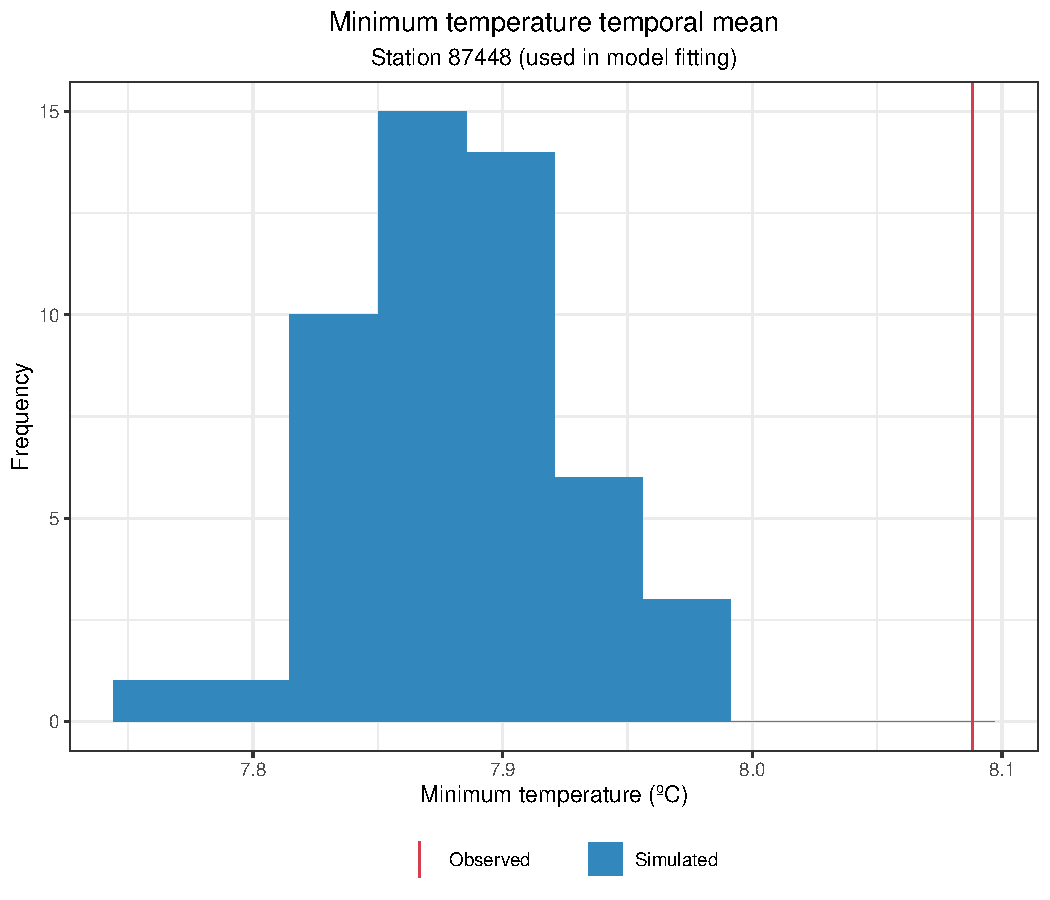
\includegraphics{Webinario_Generador_files/figure-latex/unnamed-chunk-48-1} \end{center}

Esta figura compara la temperatura mínima media de la serie observada con la de las distintas realizaciones. La línea vertical roja corresponde al valor observado mientras que las barras a las distintas realizaciones. Se observa que la medias mínimas de todos las realizaciones se encuentran en un rango muy estrecho del orden de dos décimas de grado centígrado. La diferencia entre la media observada el centro de la distribución de las medias mínimas generadas es de menos de 0.2 °C.

\begin{center}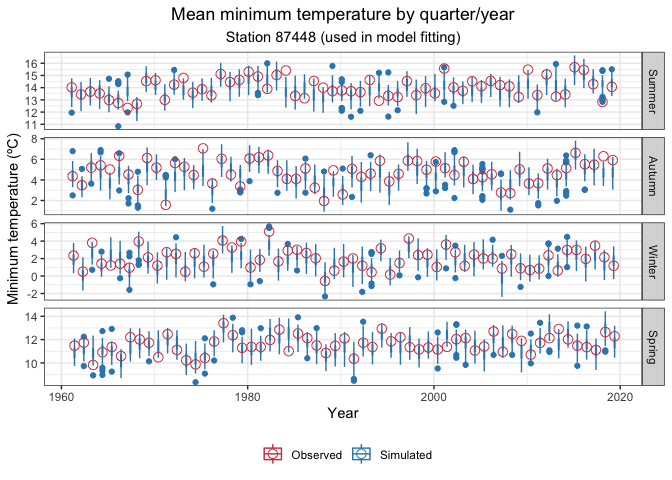
\includegraphics{Webinario_Generador_files/figure-latex/unnamed-chunk-49-1} \end{center}

Esta figura muestra la probabilidad acumulada de la temperatura mínima por trimestre del año. La línea roja corresponde a la probabilidad observada mientras que las azules, a las distintas realizaciones. Se observa que las líneas azules envuelven perfectamente a la línea roja por lo que la distribución probabilística es casi idéntica.

\begin{center}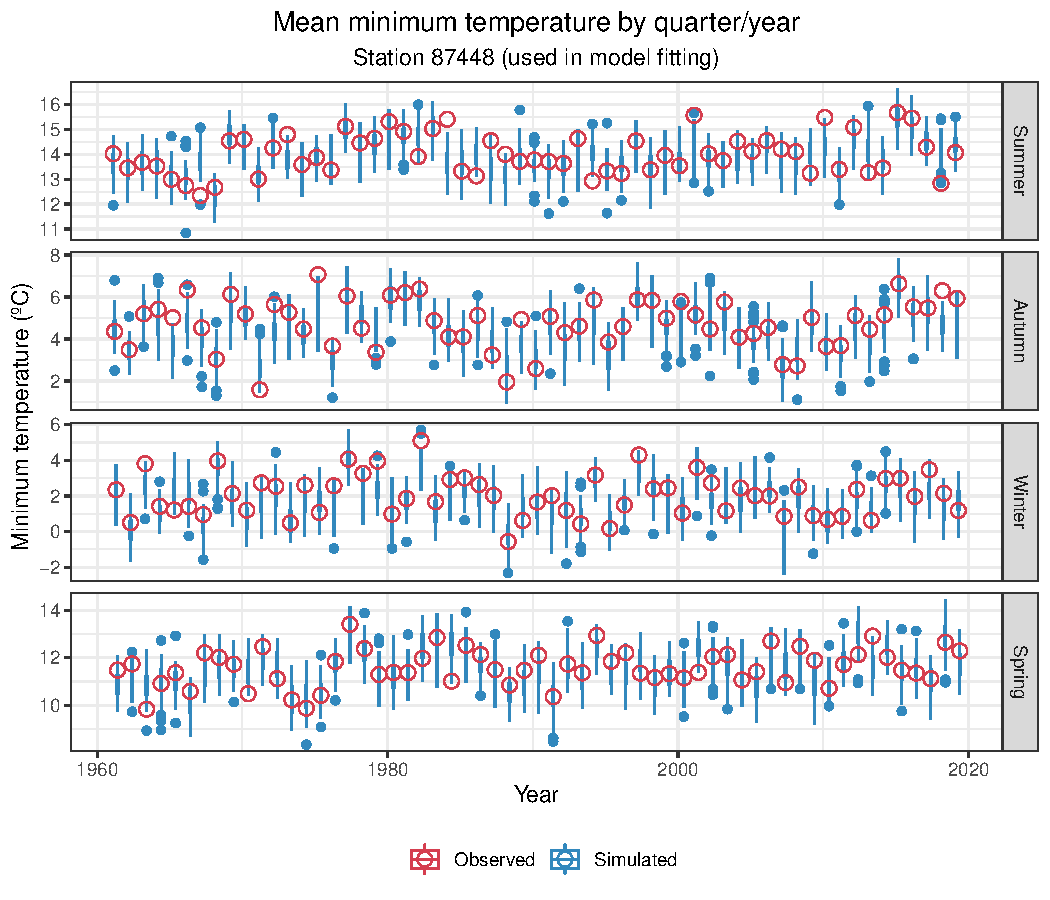
\includegraphics{Webinario_Generador_files/figure-latex/unnamed-chunk-50-1} \end{center}

Esta figura compara la variabilidad de la temperatura mínima media por trimestre a lo largo del tiempo. Los puntos rojos corresponden a las medias observadas mientras que las cajas a las distintas realizaciones. Se observa que las cajas siguen el comportamiento de los datos observados incluso en años con grandes variaciones frente a la media.

\begin{center}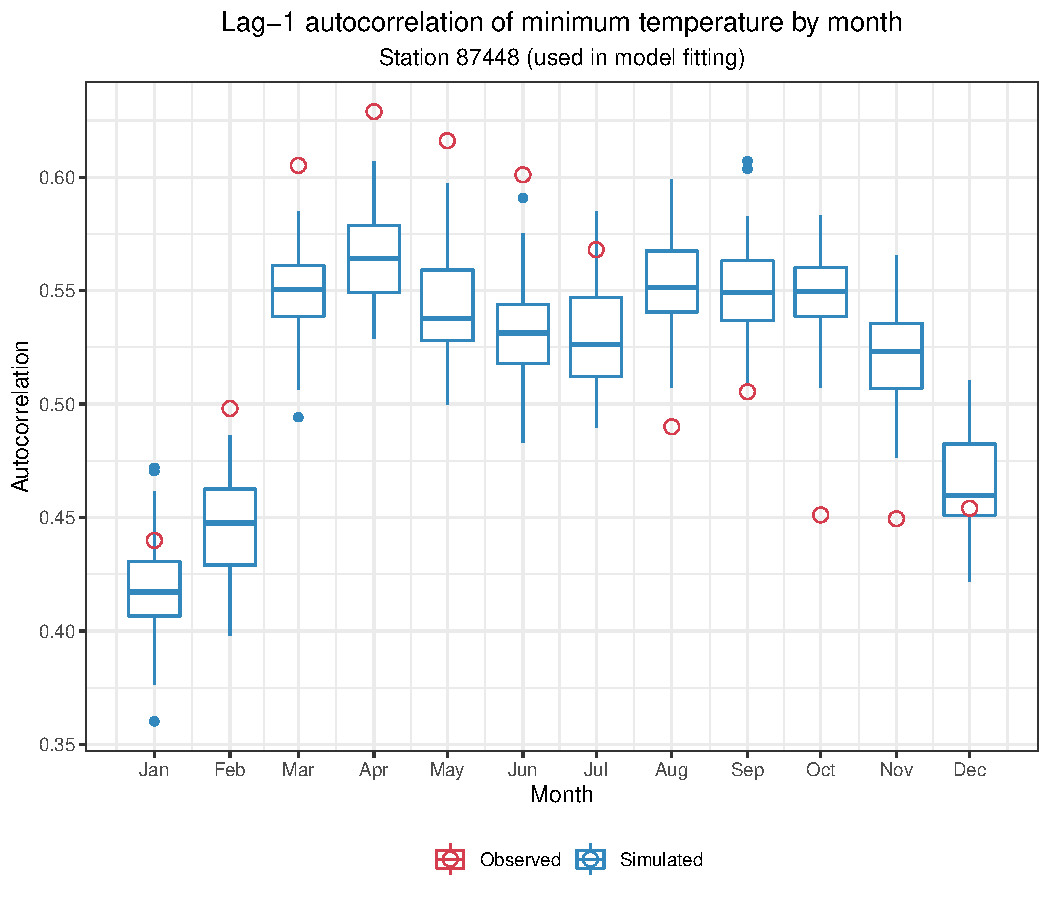
\includegraphics{Webinario_Generador_files/figure-latex/unnamed-chunk-51-1} \end{center}

Esta figura compara la autocorrelación de los valores con el lag -1. Es decir, compara la temperatura mínima diaria del día \textbf{t} con la temperatura mínima del día \textbf{t-1}. Los puntos rojos corresponden a la autocorrelación observada mientras que las cajas a las distintas realizaciones. Se observa un patrón anual muy marcado con autocorrelaciones más altas en otoño e invierno que en verano.

\begin{center}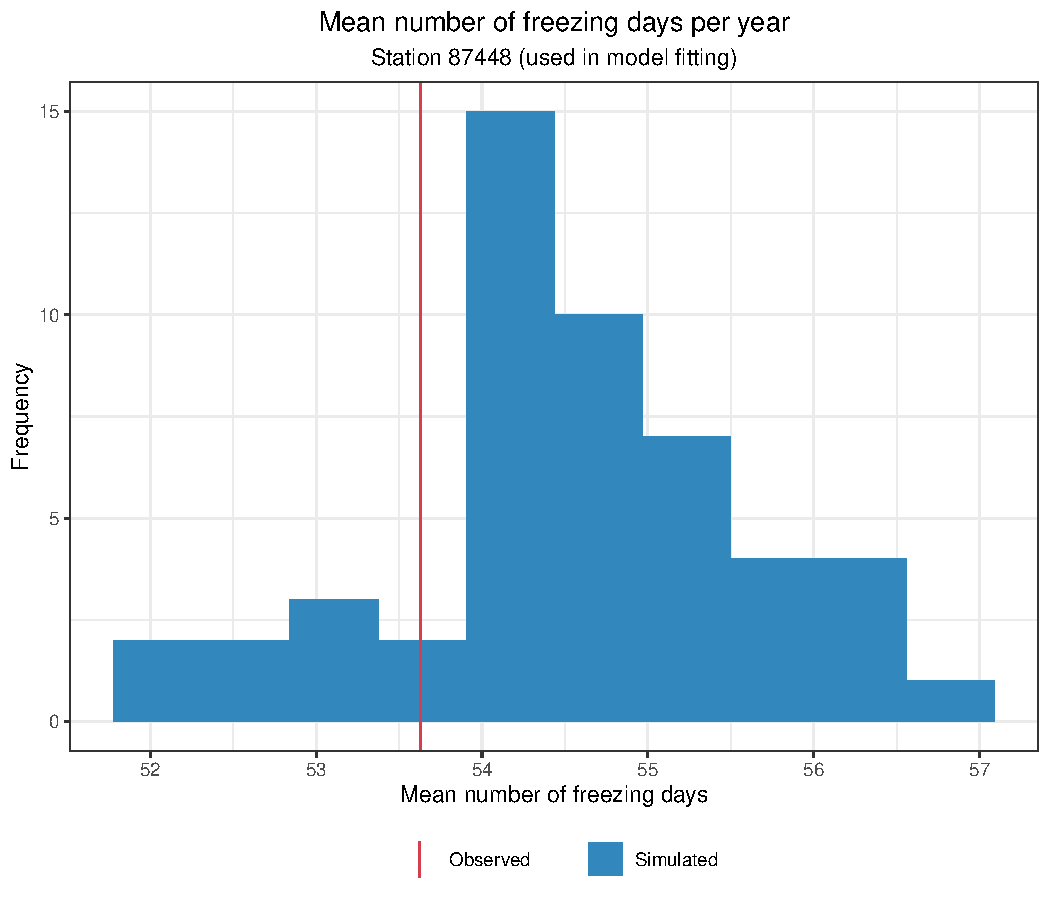
\includegraphics{Webinario_Generador_files/figure-latex/unnamed-chunk-52-1} \end{center}

Esta figura compara la cantidad de días con heladas durante un año. La línea vertical roja corresponde a la cantidad media de heladas por año calculada a partir de los registros históricos mientras que las barras corresponden a las distintas realizaciones. El generador es capaz de simular muy bien los días con heladas ya que que la diferencia entre el valor observado y la media de la distribución de las series sintéticas es menor a un día.

\begin{center}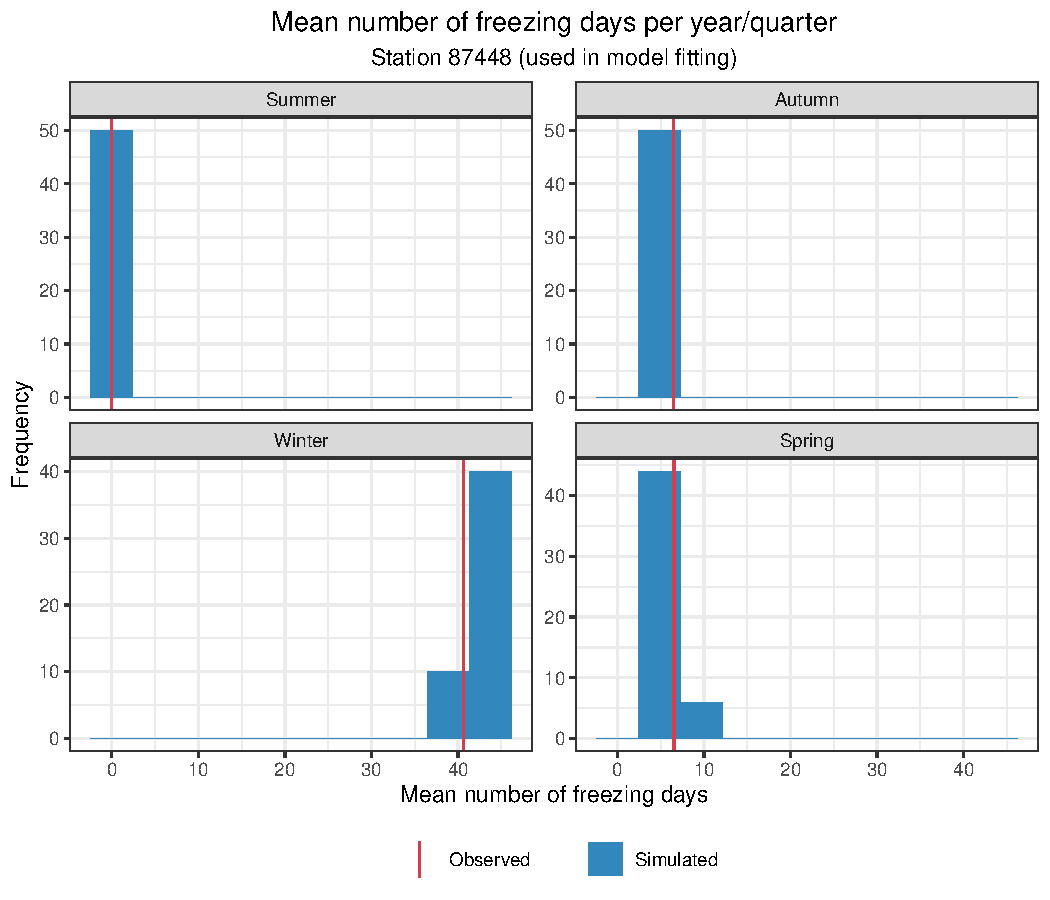
\includegraphics{Webinario_Generador_files/figure-latex/unnamed-chunk-53-1} \end{center}

Esta figura es similar a la anterior con la diferencia en que se divide el año en los distintos trimestres. Al igual que en el caso anterior, la cantidad de días con heladas generados es prácticamente idéntica a lo observado.

\begin{center}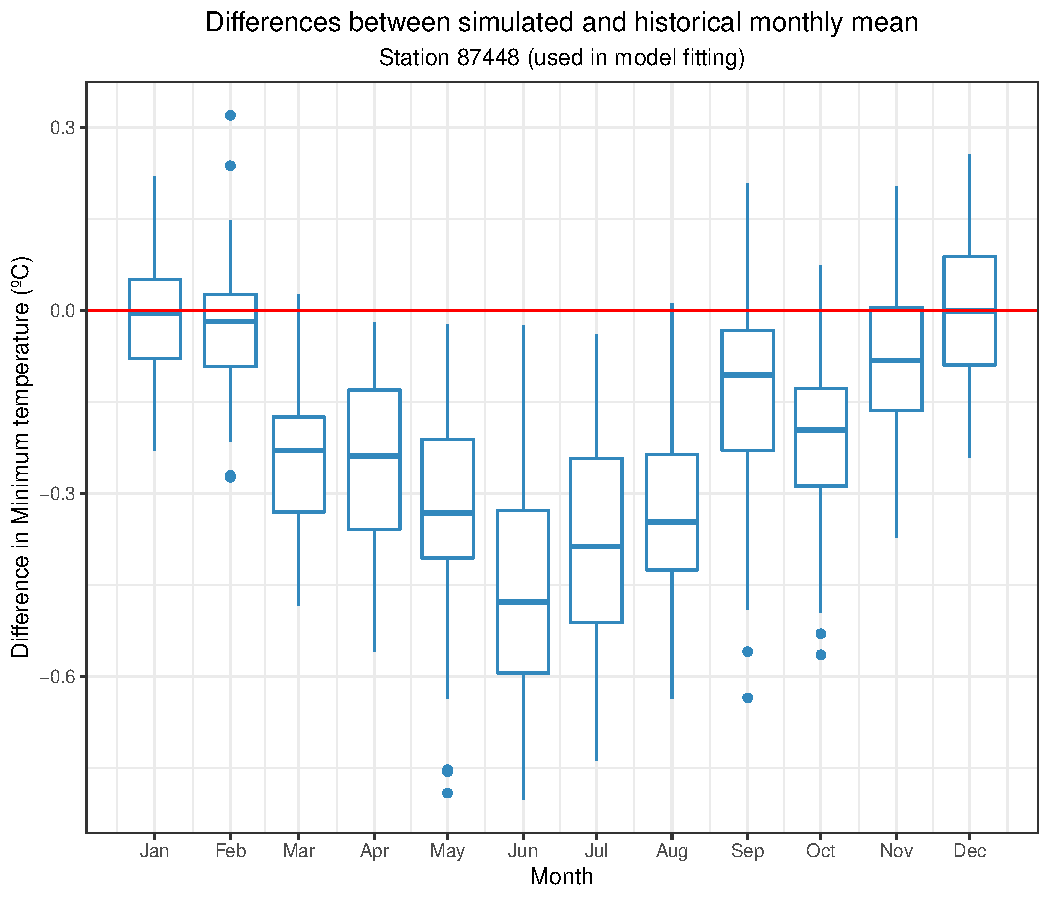
\includegraphics{Webinario_Generador_files/figure-latex/unnamed-chunk-54-1} \end{center}

Esta figura compara la media mensual calculada a partir de la series histórica con las distintas realizaciones para cada mes del año. La línea roja corresponde a una diferencia de 0 lo que quiere decir que la media observada y generada son iguales. Se observa que durante los meses invernales hay un ligero sesgo cálido de 0.5 °C aproximadamente.

\begin{center}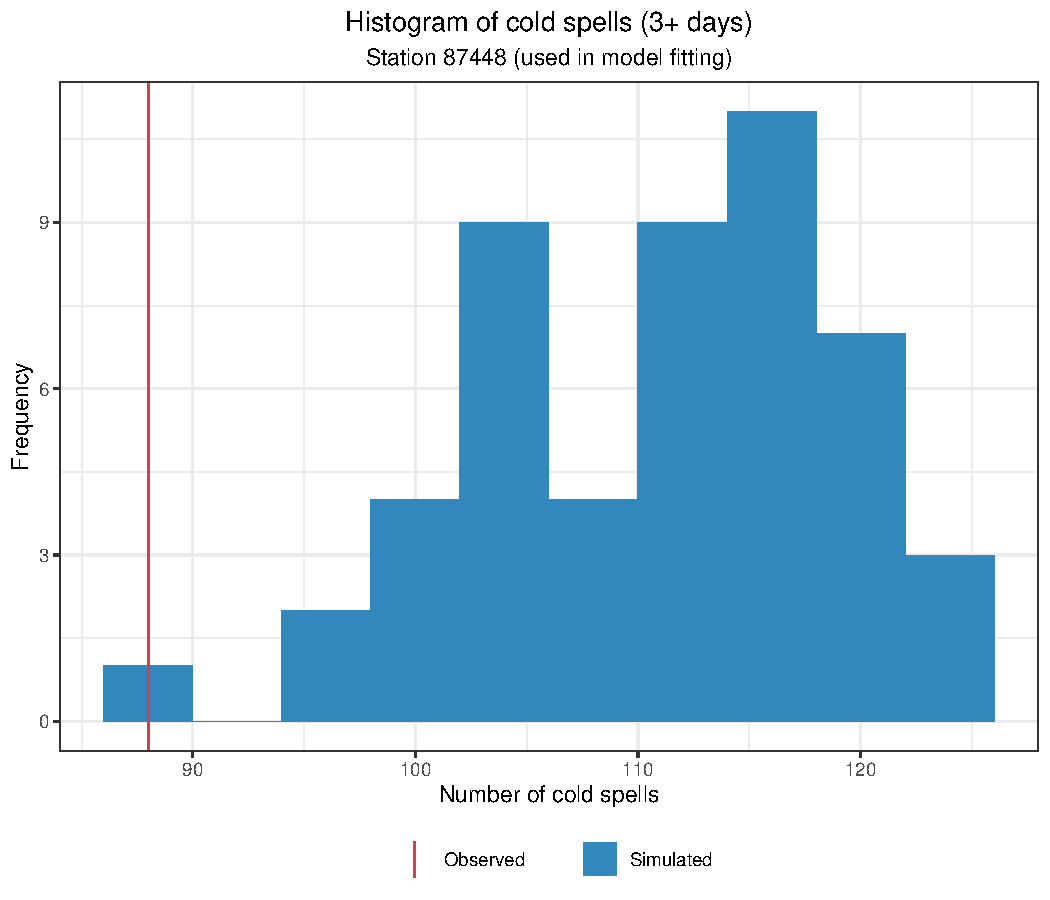
\includegraphics{Webinario_Generador_files/figure-latex/unnamed-chunk-55-1} \end{center}

Esta figura compara la distribución de la cantidad de rachas frías generadas con las observadas en el registro histórico. La línea roja corresponde a la cantidad de períodos fríos totales en el registro mientras que las barras a las distintas realizaciones. Se observa que hay una subestimación en la cantidad total de rachas cálidas para esta estación.

\hypertarget{diagnuxf3sticos-de-auxiliares}{%
\subsection{Diagnósticos de auxiliares}\label{diagnuxf3sticos-de-auxiliares}}

En esta sección se muestran de diagnósticos auxiliares centrados en la consistencia entre variables.

\begin{Shaded}
\begin{Highlighting}[]
\CommentTok{# Correlación cruzada entre las temperaturas máximas y mínimas por mes}
\NormalTok{plots[[station.id]][[}\StringTok{'other'}\NormalTok{]][[}\DecValTok{1}\NormalTok{]]}
\end{Highlighting}
\end{Shaded}

\begin{center}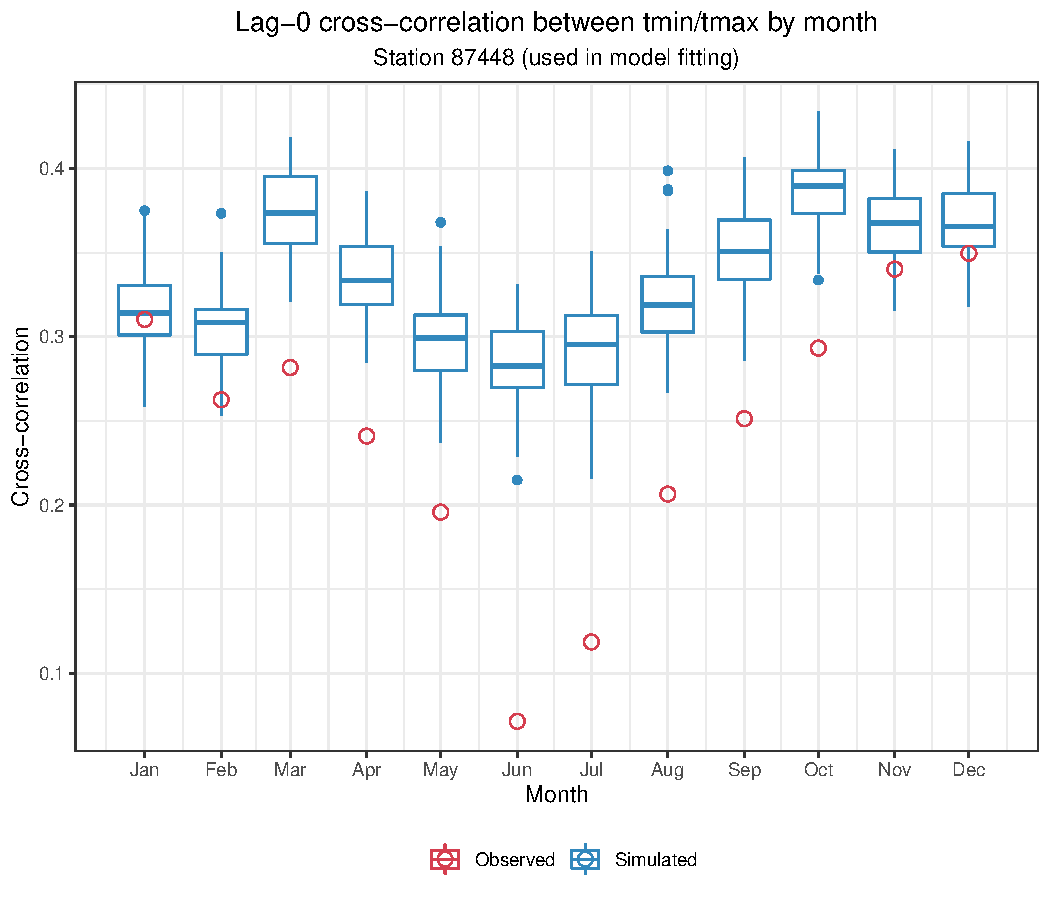
\includegraphics{Webinario_Generador_files/figure-latex/unnamed-chunk-56-1} \end{center}

Esta figura compara la variación mensual de la correlación cruzada entre las temperaturas máximas y mínimas. La autocorrelación cruzada evalúa si ambas variables varían al mismo tiempo y con que magnitud. Los puntos rojos corresponden a la correlación cruzada calculada a partir de los datos observados y las cajas a las distintas realizaciones. Se observa que se captura el patrón general aunque con una subestimación durante el invierno. Una baja autocorrelación implica grandes amplitudes térmicas ya que no varían conjuntamente.

\begin{Shaded}
\begin{Highlighting}[]
\CommentTok{# Temperatura media diaria mensual por tipo de día (seco o lluvioso)}
\NormalTok{plots[[station.id]][[}\StringTok{'other'}\NormalTok{]][[}\DecValTok{2}\NormalTok{]]}
\end{Highlighting}
\end{Shaded}

\begin{center}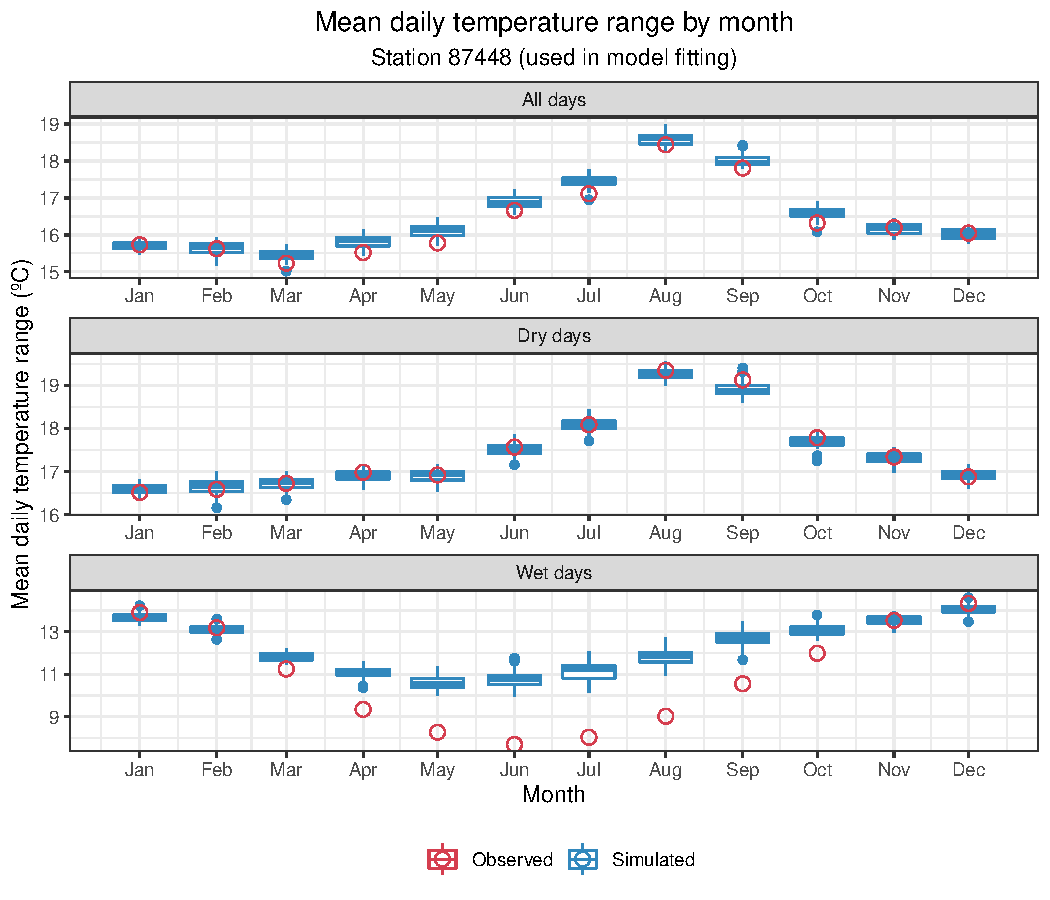
\includegraphics{Webinario_Generador_files/figure-latex/unnamed-chunk-57-1} \end{center}

Esta figura compara la temperatura media para los distintos meses del año considerando el tipo de día, es decir, si llovió o no. Los puntos rojos corresponden al valor observado mientras que las cajas a las distintas realizaciones. Se observa que cuando se consideran todos los días o sólo los días secos la concordancia es muy buena. Para los días lluviosos, en cambio, ésta sigue siendo buena para los meses estivales pero existe un marcado sesgo cálido en el invierno. Esto podría deberse a que en esta estación hay muy poco días lluviosos en invierno por lo que no son suficientes para que el modelo los capture.

\end{document}
